\documentclass[a4paper,11pt]{book}
\usepackage[centering,margin=2.5cm]{geometry}
\usepackage[export]{adjustbox}
\usepackage[utf8]{inputenc}
\usepackage[T1]{fontenc}
\usepackage{PTSerif}
\usepackage{parskip}
\usepackage{tabularx}
\usepackage{tabularray}
\usepackage{multirow}
\usepackage{float}
\usepackage{tikz}
\usetikzlibrary{shapes.geometric, arrows.meta}
\tikzstyle{textonly} = [rectangle, 
minimum width=1cm, 
minimum height=1cm,
text centered, 
draw=white]
\tikzstyle{whrectround} = [rectangle, rounded corners,
minimum width=1cm, 
minimum height=1cm, 
text centered, 
text width=2cm, 
draw=black]
\usepackage{amstext}
\usepackage{array,calc}
\newcolumntype{L}{>{$}l<{$}}
\usepackage{graphicx}
\renewcommand{\arraystretch}{1.5}
\usepackage{listings}
\usepackage{xcolor}
\definecolor{codegreen}{rgb}{0,0.6,0}
\definecolor{codegray}{rgb}{0.5,0.5,0.5}
\definecolor{codepurple}{rgb}{0.58,0,0.82}
\definecolor{backcolour}{rgb}{0.95,0.95,0.92}
\lstdefinestyle{codestyle}{
	backgroundcolor=\color{backcolour},   
	commentstyle=\color{codegreen},
	keywordstyle=\color{magenta},
	numberstyle=\tiny\color{codegray},
	stringstyle=\color{codepurple},
	basicstyle=\ttfamily\footnotesize,
	breakatwhitespace=false,         
	breaklines=true,                 
	captionpos=b,                    
	keepspaces=true,                 
	numbers=left,                    
	numbersep=5pt,                  
	showspaces=false,                
	showstringspaces=false,
	showtabs=false,                  
	tabsize=2
}
\lstset{style=codestyle}
\usepackage{amsmath}
\setcounter{MaxMatrixCols}{20}
\usepackage{longtable,booktabs}
\makeatletter
\renewcommand{\frontmatter}{\cleardoublepage\@mainmatterfalse}
\renewcommand{\mainmatter}{\cleardoublepage\@mainmattertrue}
\makeatother
\usepackage[pdftex,
			pdfauthor={Wojciech Kaczmarski SP5WWP, et al.},
			pdftitle={M17 Protocol Specification},
			pdfsubject={Protocol specification of the Amateur Radio digital mode commonly called M17},
			pdfkeywords={m17, amateur radio, ham radio, digital, digital radio, codec 2, open source, specification},
			]{hyperref}

%opening
\title{M17 Protocol Specification}
\author{Wojciech Kaczmarski, SP5WWP et al.}

\begin{document}

\begin{titlepage}
	\raggedleft
	
\includegraphics[width=0.7\linewidth,right]{img/m17_logo_shadow}
	\vspace*{\baselineskip}
	{\Large Wojciech Kaczmarski SP5WWP, et al.} \\
	\vspace*{0.167\textheight}
	\textbf{\LARGE M17 Protocol Specification} \\
	\today
	\vfill
	{\large Version 1.0}
	\vfill
	\LaTeX version compiled by Steve Miller KC1AWV
\end{titlepage}

\frontmatter

\tableofcontents

\listoftables

\listoffigures

\chapter{Licenses}

\paragraph{M17 Protocol Specification}

Copyright \copyright{}  2023  M17 Project. \\

Permission is granted to copy, distribute and/or modify this document under the terms of the GNU Free Documentation License, Version 1.3 or any later version published by the Free Software Foundation; with no Invariant Sections, no Front-Cover Texts, and no Back-Cover Texts. A copy of the license is included in the section entitled ``GNU Free Documentation License'' or at the following web page: \href{https://www.gnu.org/licenses/fdl-1.3.en.html}{https://www.gnu.org/licenses/fdl-1.3.en.html}

\paragraph{M17 Project Software}

Copyright (C) 2023  M17 Project \\

Software included in the M17 Protocol Specification is free software; you can redistribute it and/or modify it under the terms of the GNU General Public License as published by the Free Software Foundation; either version 2 of the License, or (at your option) any later version.

This program is distributed in the hope that it will be useful, but WITHOUT ANY WARRANTY; without even the implied warranty of MERCHANTABILITY or FITNESS FOR A PARTICULAR PURPOSE.  See the GNU General Public License for more details.

You should have received a copy of the GNU General Public License along with this program; if not, write to the Free Software Foundation, Inc., 51 Franklin Street, Fifth Floor, Boston, MA  02110-1301, USA.

\chapter{Introduction}

M17 is an RF protocol that is:

\begin{itemize}
	\item
	Completely open: open specification, open source code, open source hardware, open algorithms. Anyone must be able to build an M17 radio  and interoperate with other M17 radios without having to pay anyone else for the right to do so.
	\item
	Optimized for amateur radio use.
	\item
	Simple to understand and implement.
	\item
	Capable of doing the things hams expect their digital protocols to do:
	\begin{itemize}
		\item
		Voice (eg: DMR, D-Star, etc)
		\item
		Point to point data (eg: Packet, D-Star, etc)
		\item
		Broadcast telemetry (eg: APRS, etc)
		\item
		Extensible, so more capabilities can be added over time.
	\end{itemize}
\end{itemize}

To do this, the M17 protocol is broken down into three protocol layers,
like a network:

\begin{enumerate}
	\def\labelenumi{\arabic{enumi}.}
	\item
	Physical Layer: How to encode 1s and 0s into RF\@. Specifies RF modulation, symbol rates, bits per symbol, etc.
	\item
	Data Link Layer: How to packetize those 1s and 0s into usable data. Packet vs Stream modes, headers, addressing, etc.
	\item
	Application Layer: Accomplishing activities. Voice and data streams, control packets, beacons, etc.
\end{enumerate}

This document attempts to document these layers.

\chapter{Glossary}

\textbf{Common terms used in M17}

\paragraph{ECC}

Error Correcting Code

\paragraph{FEC}

Forward Error Correction

\paragraph{Frame}

The individual components of a stream, each of which contains payload data interleaved with frame signalling.

\paragraph{Link Setup Frame}

The first frame of any transmission. It contains full link information
data.

\paragraph{LICH}

Link Information Channel. The LICH contains all information needed to establish an M17 link. The first frame of a transmission contains full LICH data, and subsequent frames each contain one sixth of the LICH data so that late-joiners can obtain the LICH\@.

\paragraph{Packet}

A single burst of transmitted data containing 100s to 1000s of bytes, after which the physical layer stops sending data.

\paragraph{Superframe}

A set of six consecutive frames which collectively contain full LICH
data are grouped into a superframe.

\mainmatter
\chapter{Physical Layer}

This section describes the M17 standard radio physical layer suitable
for use where a transmission bandwidth of 9 kHz is permitted.

\section{4-level Frequency-shift Keying Modulation (4FSK)}

The M17 standard uses 4FSK at 4800 symbols/s (9600 bits/s) with a deviation index h=1/3 for transmission in a 9 kHz channel bandwidth. Minimum channel spacing is 12.5 kHz.

\section{Dibit, Symbol, and Frequency-shift}

Each of the 4-level frequency-shifts can be represented by dibits (2-bit values) or symbols, as shown in Table 1 below.

In the case of dibits, the most significant bit is sent first. When four dibits are grouped into a byte, the most significant dibit of the byte
is sent first. For example, the four dibits contained in the byte \texttt{0xB4} (0b 10 11 01 00) would be sent as the symbols (-1, -3, +3, +1).

\begin{table}[H]
	\centering
	\begin{tabular}{|c|c|c|c|}
		\hline
		\multicolumn{2}{|c|}{Dibit} & \multirow{2}{*}{Symbol} & \multirow{2}{*}{Deviation} \\
		MSB & LSB &  &  \\
		\hline
		0 & 1 & +3 & +2.4 kHz \\
		0 & 0 & +1 & +0.8 kHz \\
		1 & 0 & -1 & -0.8 kHz \\
		1 & 1 & -3 & -2.4 kHz \\
		\hline
	\end{tabular}
	\caption{Dibit symbol mapping to 4FSK deviation}
\end{table}

\section{4FSK Generation}

\begin{center}
	\begin{figure}[H]
	
\begin{tikzpicture}[node distance=2cm]
		\node (in) [textonly] {Dibit Input};
		\node (sym) [whrectround, right of=in, xshift=1cm] {Dibit to Symbol};
		\node (up) [whrectround, right of=sym, xshift=1cm] {Upsampler};
		\node (rrc) [whrectround, right of=up, xshift=1cm] {RRC Filter};
		\node (fm) [whrectround, right of=rrc, xshift=1cm] {Frequency Modulation};
		\node (out) [textonly, right of=fm, xshift=1cm] {4FSK Output};
		
		\draw [-latex](in) -- (sym);
		\draw [-latex](sym) -- (up);
		\draw [-latex](up) -- (rrc);
		\draw [-latex](rrc) -- (fm);
		\draw [-latex](fm) -- (out);
	\end{tikzpicture}
	\caption{4FSK Generation}
	\end{figure}
\end{center}

Dibits are converted to symbols. The symbol stream is upsampled to a series of impulses which pass through a root-raised-cosine (alpha=0.5) shaping filter before frequency modulation at the transmitter and again after frequency demodulation at the receiver.

Upsampling by a factor of 10 is recommended (48000 samples/s).

The root-raised-cosine filter should span at least 8 symbols (81 taps at the recommended upsample rate).

\section{Transmission}

A complete transmission shall consist of a Preamble, a Synchronization Burst, Payload, and an End of Transmission marker.

\begin{table}[H]
	\centering
	\begin{tabular}{cccc}
		\hline
		\multicolumn{1}{|c|}{PREAMBLE} & \multicolumn{1}{c|}{SYNC BURST} & \multicolumn{1}{c|}{PAYLOAD} & \multicolumn{1}{c|}{EoT} \\ \hline
		\begin{tabular}[c]{@{}c@{}}40ms\\ (192 symbols)\end{tabular} & \begin{tabular}[c]{@{}c@{}}16 bits\\ (8 symbols)\end{tabular} & \begin{tabular}[c]{@{}c@{}}Multiples of 2 bits\\ (multiples of 1 symbol)\end{tabular} & \begin{tabular}[c]{@{}c@{}}40ms\\ (192 symbols)\end{tabular}
	\end{tabular}
	\caption{Physical Layer Transmission}
\end{table}

Transmissions may include more than one synchronization burst followed by a payload.

\begin{table}[H]
	\centering
	\begin{tblr}{|l|l|l|[dashed]l|[dashed]l|l|l|}
		\hline
		PREAMBLE & SYNC BURST & PAYLOAD & ••• & SYNC BURST & PAYLOAD & EoT \\ \hline
	\end{tblr}
	\caption{Physical Layer Transmission with Multiple Synchronization Bursts}
\end{table}

\subsection{Preamble}

Every transmission shall start with a preamble, which shall consist of 40 ms (192 symbols) of alternating outer symbols (+3, -3) or (-3, +3). To ensure a zero crossing prior to a synchronization burst, the last symbol transmitted within the preamble shall be opposite the first symbol transmitted in the synchronization burst.

\subsection{Synchronization Burst (Sync Burst)}

A sync burst of 16 bits (8 symbols) shall be sent immediately after the preamble. The sync burst is constructed using only outer symbols, with codings based on \href{https://en.wikipedia.org/wiki/Barker_code}{Barker codes}. Properly chosen sync burst coding assists in symbol clocking and alignment. Different sync burst codes may also be used by the Data Link Layer to identify the type of payload to follow.

\subsection{Payload}

Payload shall be transmitted in multiples of 2 bits (1 symbol).

\subsection{Randomizer}

To avoid transmitting long sequences of constant symbols (e.g.~+3, +3, +3, \ldots), a simple randomizing algorithm is used. At the transmitter, all payload bits shall be XORed with a pseudorandom predefined sequence before being converted to symbols. At the receiver, the randomized payload symbols are converted to bits and are again passed through the same XOR algorithm to obtain the original payload bits.

The pseudorandom sequence is composed of the 46 bytes (368 bits) found in the appendix Randomizer Sequence.

Before each bit of payload is converted to symbols for transmission, it is XORed with a bit from the pseudorandom sequence. The first payload bit is XORed with most significant bit (bit 7) of sequence byte 0 \texttt{(0$\times$D6)}, second payload bit with bit 6 of sequence byte 0, continuing to the eighth payload bit and bit 0 of sequence byte 0. The ninth payload bit is XORed with bit 7 of sequence byte 1 \texttt{(0$\times$B5)}, tenth payload bit with bit 6 of sequence byte 1, etc.

When payload bits have XORed through sequence byte 45 \texttt{(0$\times$C3)}, the pseudorandom sequence is restarted at sequence byte 0 \texttt{(0$\times$D6)}.

On the receive side, symbols are converted to randomized payload bits. Each randomized payload bit is converted back to a payload bit by once
again XORing each randomized bit with the corresponding pseudorandom sequence bit.

\subsection{End of Transmission marker (EoT)}

Every transmission ends with a distinct symbol stream, which shall consist of 40 ms (192 symbols) of a repeating \texttt{(0$\times$55)} \texttt{(0$\times$5D)} (+3, +3, +3, +3, +3, +3, -3, +3) pattern.

\subsection{Carrier-sense Multiple Access (CSMA)}

CSMA may be used to minimize collisions on a shared radio frequency by having the sender ensure the frequency is clear before transmitting. Higher layers (Data Link and Application) may require the use of CSMA, and may specify parameters other than the defaults.

\href{https://en.wikipedia.org/wiki/Carrier-sense_multiple_access}{P-persistent} access is used with a default probability of p = 0.25 and default slot time of 40 ms.

\section{Physical Layer Flow Summary}

\begin{figure}[H]
	\centering
	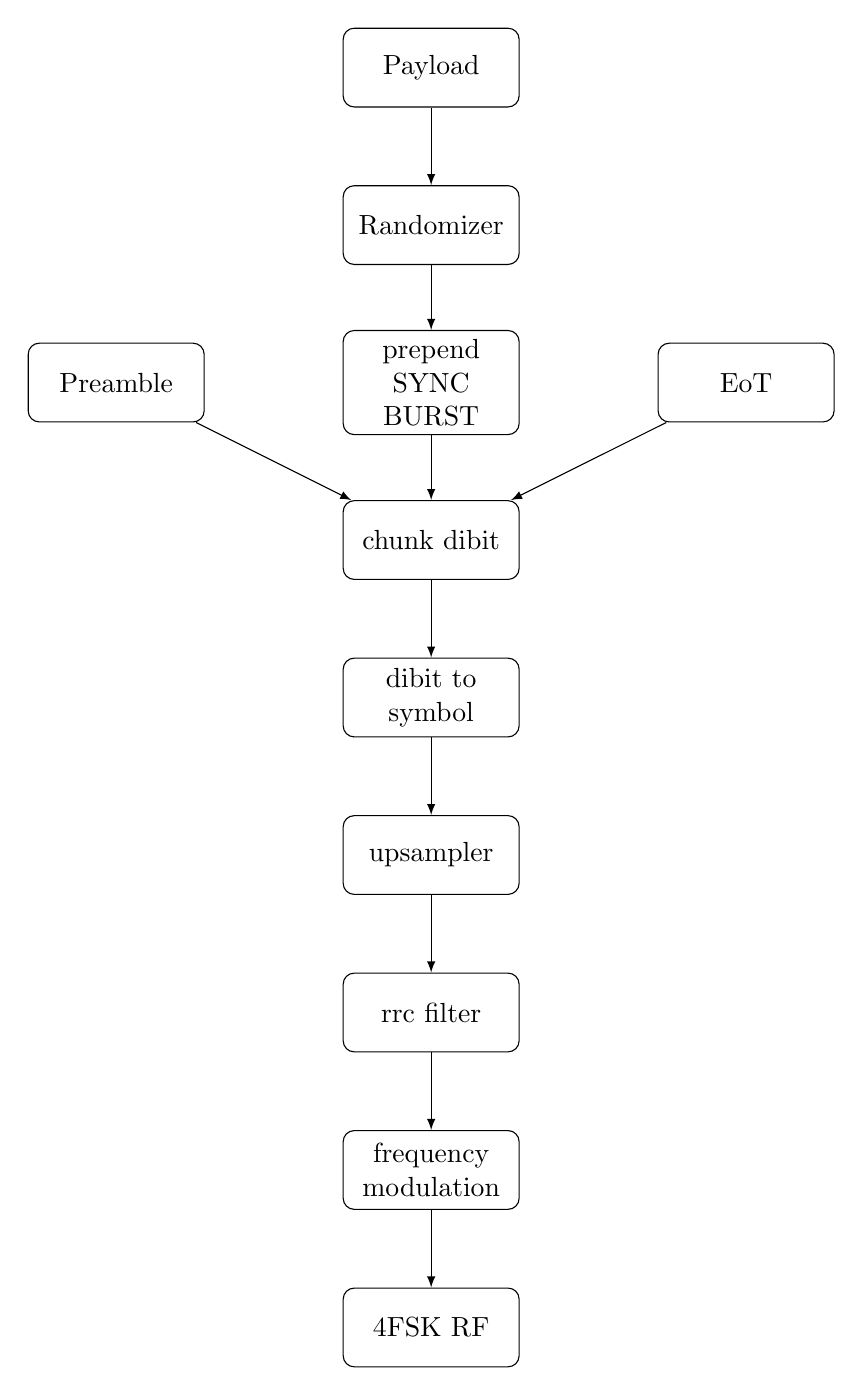
\begin{tikzpicture}[node distance=2cm]
		\node (payload) [whrectround] {Payload};
		\node (rand) [whrectround, below of=payload] {Randomizer};
		\node (sync) [whrectround, below of=rand] {prepend SYNC BURST};
		\node (pre) [whrectround, left of=sync, xshift=-2cm] {Preamble};
		\node (eot) [whrectround, right of=sync, xshift=2cm] {EoT};
		\node (cd) [whrectround, below of=sync] {chunk dibit};
		\node (dtos) [whrectround, below of=cd] {dibit to symbol};
		\node (up) [whrectround, below of=dtos] {upsampler};
		\node (rrc) [whrectround, below of=up] {rrc filter};
		\node (fm) [whrectround, below of=rrc] {frequency modulation};
		\node (fsk) [whrectround, below of=fm] {4FSK RF};
		
		\draw [-latex](payload) -- (rand);
		\draw [-latex](rand) -- (sync);
		\draw [-latex](sync) -- (cd);
		\draw [-latex](pre) -- (cd);
		\draw [-latex](eot) -- (cd);
		\draw [-latex](cd) -- (dtos);
		\draw [-latex](dtos) -- (up);
		\draw [-latex](up) -- (rrc);
		\draw [-latex](rrc) -- (fm);
		\draw [-latex](fm) -- (fsk);
	\end{tikzpicture}
	\caption{Physical Layer Flow}
\end{figure}

\chapter{Data Link Layer}

\section{Frame}

A Frame shall be composed of a frame type specific Synchronization Burst (Sync Burst) followed by 368 bits (184 symbols) of Payload. The combination of Sync Burst plus Payload results in a constant 384 bit (192 symbol) Frame. At the M17 data rate of 4800 symbols/s (9600 bits/s), each Frame is exactly 40ms in duration.

There are four frame types each with their own specific Sync Burst: Link Setup Frames (LSF), Bit Error Rate Test (BERT) Frames, Stream Frames, and Packet Frames.

\begin{table}[H]
	\centering
	\begin{tabular}{cc}
		\hline
		\multicolumn{1}{|c|}{SYNC BURST} & \multicolumn{1}{c|}{PAYLOAD} \\ \hline
		\begin{tabular}[c]{@{}c@{}}16 bits\\ (8 symbols)\end{tabular} & \begin{tabular}[c]{@{}c@{}}368 bits\\ (184 symbols)\end{tabular}
	\end{tabular}
	\caption{Frame}
\end{table}

\section{Forward Error Correction (FEC)}

The Data Link Layer Contents of a specific frame are modified using various Error Correction Code (ECC) methods. Applying these codes at the transmitter allows the receiver to correct some amount of induced errors in a Forward Error Correction (FEC) process. It is this ECC/FEC data that is inserted into the Payload portion of the Frame. The exact ECC/FEC techniques used vary by frame type.

Applying ECC/FEC may be a multi-step process. To distinguish data bits at the various stages of the process, Bit Types are defined as shown in the following table. It is important to note that not all ECC/FEC processes utilize both Type 2 and Type 3 bits. Prior to decoding Data Link Layer contents, a receiver would need to convert incoming bits from Type 4 back to Type 1 bits, which may also include conversion through Type 3 and/or Type 2 bits. The exact ECC/FEC methods and Bit Types
utilized will be indicated for each frame type.

\begin{table}[H]
	\centering
	\begin{tblr}{
		colspec={lX},
		}
		\hline
		Type & Description \\
		\hline
		Type 1 & Data link layer content bits \\
		Type 2 & Bits after appropriate encoding \\
		Type 3 & Bits after puncturing \\
		Type 4 & Interleaved (re-ordered) bits \\
		\hline[2px]
	\end{tblr}
	\caption{Bit Types}
\end{table}

\begin{figure}[H]
	\centering
	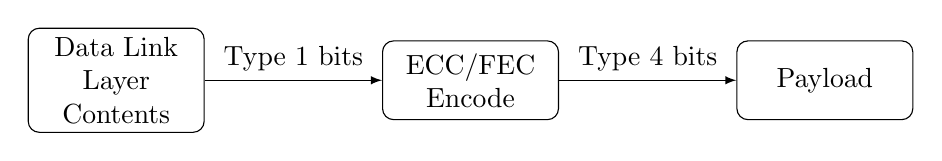
\begin{tikzpicture}[node distance=2cm]
		\node (cont) [whrectround] {Data Link Layer Contents};
		\node (ecc) [whrectround, right of=cont, xshift=2.5cm] {ECC/FEC Encode};
		\node (payload) [whrectround, right of=ecc, xshift=2.5cm] {Payload};
		
		\draw [-latex](cont) -- node [midway, above] {Type 1 bits} (ecc);
		\draw [-latex](ecc) -- node [midway, above] {Type 4 bits} (payload);
	\end{tikzpicture}
	\caption{Transmit Contents to Payload}
\end{figure}

\begin{figure}[H]
	\centering
	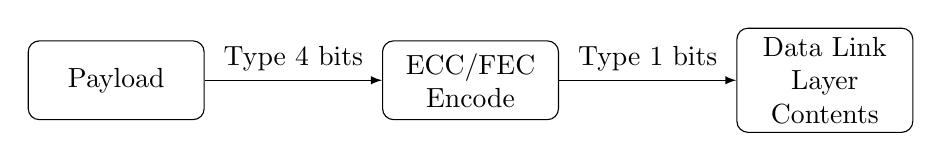
\begin{tikzpicture}[node distance=2cm]
		\node (payload) [whrectround] {Payload};
		\node (ecc) [whrectround, right of=payload, xshift=2.5cm] {ECC/FEC Encode};
		\node (cont) [whrectround, right of=ecc, xshift=2.5cm] {Data Link Layer Contents};
		
		\draw [-latex](payload) -- node [midway, above] {Type 4 bits} (ecc);
		\draw [-latex](ecc) -- node [midway, above] {Type 1 bits} (cont);
	\end{tikzpicture}
	\caption{Receive Payload to Contents}
\end{figure}

\section{Modes}

The Data Link layer shall operate in one of three modes during a Transmission.

\begin{itemize}
	\item
	Stream Mode
    Data are sent in a continuous stream for an indefinite amount of time, with no break in physical layer output, until the stream ends. e.g.~voice data, bulk data transfers, etc. Stream Mode shall start with an LSF and is followed by one or more Stream Frames.
	\item
	Packet Mode
	Data are sent in small bursts, up to 798 bytes at a time, after which the physical layer stops sending data. e.g.~messages, beacons, etc. Packet Mode shall start with an LSF and is followed by one to 32 Packet Frames.
	\item
	BERT Mode
	PRBS9 is used to fill frames with a deterministic bit sequence. Frames are sent in a continuous sequence. Bert Mode shall start with a BERT frame, and is followed by one or more BERT Frames.
\end{itemize}

\begin{quote}
	NOTE As is the convention with other networking protocols, all values and data structures are encoded in big endian byte order.
\end{quote}

\section{Synchronization Burst (Sync Burst)}

All frames shall be preceded by 16 bits (8 symbols) of
Sync Burst. The Sync Burst definition straddles both the Physical Layer and the Data Link Layer.

Only LSF and BERT Sync Bursts may immediately follow the Preamble, and each requires a different Preamble symbol pattern as shown in the table below.

During a Transmission, only one LSF Sync Burst may be present, and if present, it shall immediately follow the Preamble.

BERT Sync Bursts, if present, may only follow the Preamble or other BERT frames.

Multiple Stream or Packet Sync Bursts may be present during a Transmission, depending on the mode.

\begin{table}[H]
	\centering
	\begin{tblr}{
		colspec={lccX},
		}
		\hline
		Frame Type & Preamble & Sync Burst Bytes & Sync Burst Symbols \\
		\hline
		LSF & +3, -3 & 0x55 0xF7 & +3, +3, +3, +3, -3, -3, +3, -3 \\
		BERT & -3, +3 & 0xDF 0x55 & -3, +3, -3, -3, +3, +3, +3, +3 \\
		Stream & None & 0xFF 0x5D & -3, -3, -3, -3, +3, +3, -3, +3 \\
		Packet & None & 0x75 0xFF & +3, -3, +3, +3, -3, -3, -3, -3 \\
		\hline[2px]
	\end{tblr}
	\caption{Frame Specific Sync Bursts}
\end{table}

\section{Link Setup Frame (LSF)}

The LSF is the initial frame for both Stream and Packet Modes and contains information needed to establish a link.

\begin{table}[H]
	\centering
	\begin{tblr}{
		colspec={lcX},
		}
		\hline
		Field & Length & Description \\
		\hline
		DST & 48 bits & Destination address - Encoded callsign or a special number (eg. a group) \\
		SRC & 48 bits & Source address - Encoded callsign of the originator or a special number (eg. a group) \\
		TYPE & 16 bits & Information about the incoming data stream \\
		META & 112 bits & Metadata field, suitable for cryptographic metadata like IVs or single-use numbers, or non-crypto metadata like the sender's GNSS position. \\
		CRC & 16 bits & CRC for the link setup data \\
		\hline[2pt]
	\end{tblr}
	\caption{Link Setup Frame Contents}
\end{table}

Total: 240 Type 1 bits

\subsection{LSF DST and SRC}

Destination and source addresses may be encoded amateur radio callsigns, or special numbers. See the Address Encoding Appendix for details.

\subsection{LSF TYPE}

The TYPE field contains information about the frames to follow LSF. The Packet/Stream indicator bit determines which mode (Packet or Stream) will be used during the transmission. The remaining field meanings are defined by the specific mode and application.

\begin{table}[H]
	\centering
	\begin{tblr}{
		colspec={lX},
		}
		\hline
		Bits & Content \\
		\hline
		0 & Packet/Stream indicator \\
		1..2 & Data type indicator \\
		3..4 & Encryption type \\
		5..6 & Encryption subtype \\
		7..10 & Channel Access Number (CAN) \\
		11..15 & Reserved (don't care) \\
		\hline[2px]
	\end{tblr}
	\caption{LSF TYPE definition}
\end{table}

\begin{table}[H]
	\centering
	\begin{tblr}{
		colspec={lX},
		}
		\hline
		Value & Mode \\
		\hline
		0 & Packet mode \\
		1 & Stream mode \\
		\hline[2px]
	\end{tblr}
	\caption{Packet/Stream indicator}
\end{table}

\begin{table}[H]
	\centering
	\begin{tblr}{
		colspec={lX},
		}
		\hline
		Value & Content \\
		\hline
		$(00_2)$ & Reserved \\
		$(01_2)$ & Data \\
		$(10_2)$ & Voice \\
		$(11_2)$ & Voice+Data \\
		\hline[2px]
	\end{tblr}
	\caption{Data type}
\end{table}

\begin{table}[H]
	\centering
	\begin{tblr}{
		colspec={lX},
		}
		\hline
		Value & Encryption \\
		\hline
		$(00_2)$ & None \\
		$(01_2)$ & Scrambler \\
		$(10_2)$ & AES \\
		$(11_2)$ & Other/reserved \\
		\hline[2px]
	\end{tblr}
	\caption{Encryption type}
\end{table}

For the encryption subtype, meaning of values depends on encryption type.

\subsection{LSF META}

The LSF META field is defined by the specific application.

\subsection{LSF CRC}

M17 uses a non-standard version of 16-bit CRC with polynomial $x^{16} + x^{14} + x^{12} + x^{11} + x^8 + x^5 + x^4 + x^2 + 1$ or \texttt{0$\times$5935} and initial value of \texttt{0$\times$FFFF}. This polynomial allows for detecting all errors up to hamming distance of 5 with payloads up to 241 bits, which is less than the amount of data in each frame.

As M17's native bit order is most significant bit first, neither the input nor the output of the CRC algorithm gets reflected.

The input to the CRC algorithm consists of DST, SRC (each 48 bits), 16 bits of TYPE field and 112 bits META, and then depending on whether the CRC is being computed or verified either 16 zero bits or the received CRC.

The test vectors in the following table are calculated by feeding the given message and then 16 zero bits to the CRC algorithm.

\begin{table}[H]
	\centering
	\begin{tblr}{
		colspec={lX},
		}
		\hline
		Message & CRC Output \\
		\hline
		(empty string) & 0xFFFF \\
		ASCII string ``A'' & 0x206E \\
		ASCII string ``123456789'' & 0x772B \\
		Bytes 0x00 to 0xFF & 0x1C31 \\
		\hline[2px]
	\end{tblr}
	\caption{CRC Test Vectors}
\end{table}

\subsection{LSF Contents ECC/FEC}

The 240 Type 1 bits of the Link Setup Frame Contents along with 4 flush bits are convolutionally coded using a rate 1/2 coder with constraint K=5. 244 bits total are encoded resulting in 488 Type 2 bits.

Type 3 bits are computed by $P_1$ puncturing the Type 2 bits, resulting in 368 Type 3 bits.

Interleaving the Type 3 bits produces 368 Type 4 bits that are ready to be passed to the Physical Layer.

Within the Physical Layer, the 368 Type 4 bits are randomized and combined with the 16-bit LSF Sync Burst, which results in a complete frame of 384 bits (384 bits / 9600bps = 40 ms).

\begin{figure}[H]
	\centering
	\begin{tikzpicture}[node distance=2cm]
		\tikzstyle{sub} = [draw,rectangle,fill=black!20]
		\node (dl) [sub] {
			\begin{tikzpicture}
				\node (dll) [rectangle,inner ysep=0cm] {Data Link Layer};
				\node (cont) [rectangle,draw,fill=white,yshift=-1cm] {Contents};
				\node (add) [rectangle,draw,below of=cont,fill=white] {add 4 flush bits};
				\node (conv) [rectangle,draw,below of=add,fill=white,yshift=1cm] {convolutional encoder};
				\node (p1) [rectangle,draw,below of=conv,fill=white] {$P_1$ puncturer};
				\node (int) [rectangle,draw,below of=p1,fill=white] {interleaver};
				\draw [-latex](cont) -- node [midway,fill=black!20] {240 Type 1 bits} (add);
				\draw [-latex](add) -- (conv);
				\draw [-latex](conv) -- node [midway,fill=black!20] {488 Type 2 bits} (p1);
				\draw [-latex](p1) -- node [midway,fill=black!20] {368 Type 3 bits} (int);
			\end{tikzpicture}
		};
		\node (pl) [sub,below of=dl,yshift=-6cm] {
			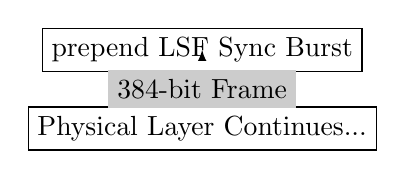
\begin{tikzpicture}
				\node (pll) [rectangle,inner ysep=0cm] {Physical Layer};
				\node (rand) [rectangle,draw,below of=pll,fill=white,yshift=1cm] {randomizer};
				\node (pre) [rectangle,draw,below of=rand,fill=white,yshift=1cm] {prepend LSF Sync Burst};
				\node (con) [rectangle,draw,below of=pre,fill=white] {Physical Layer Continues...};
				\draw [-latex](rand) -- (pre);
				\draw [-latex](pre) -- node [midway,fill=black!20] {384-bit Frame} (con);
			\end{tikzpicture}
		};
		\draw [-latex](dl) -- node [midway,fill=white] {368 Type 4 bits} (pl);
	\end{tikzpicture}
	\caption{LSF Construction}
\end{figure}

\section{Stream Mode}

In Stream Mode, an \emph{indefinite} amount of data is sent continuously
without breaks in the physical layer. Stream Mode shall always start
with an LSF that has the LSF TYPE Packet/Stream indicator bit set to 1
(Stream Mode). Other valid LSF TYPE parameters are selected per
application.

Following the LSF, one or more Stream Frames may be sent.

\begin{table}[H]
	\centering
	\begin{tblr}{
			colspec={|c|X[c]|X[c]|X[c]|X[c]|[dashed]c|[dashed]X[c]|X[c]|c|},
			rows={m},
			hlines,
		}
		PREAMBLE & LSF SYNC BURST & LSF FRAME & STREAM SYNC BURST & STREAM FRAME & ••• & STREAM SYNC BURST & STREAM FRAME & EoT \\
	\end{tblr}
	\caption{Stream Mode}
\end{table}

\subsection{Stream Frames}

Stream Frames are composed of frame signalling information contained within the Link Information Channel (LICH) combined with Stream Contents. Both the LICH and Stream Contents utilize different ECC/FEC mechanisms, and are combined at the bit level in a Frame Combiner.

\paragraph{Link Information Channel (LICH)}

The LICH allows for late listening and independent decoding to check destination address if the LSF for the current transmission was missed.

Each Stream Frame contains a 48-bit Link Information Channel (LICH). Each LICH within a Stream Frame includes a 40-bit chunk of the 240-bit LSF frame that was used to establish the stream. A 3-bit modulo 6 counter (LICH\_CNT) is used to indicate which chunk of the LSF is present in the current Stream Frame. LICH\_CNT starts at 0, increments to 5, then wraps back to 0.

\begin{table}[H]
	\centering
	\begin{tblr}{
		colspec={lX},
		}
		\hline
		Bits & Content \\
		\hline
		0..39 & 40-bit chunk of full LSF Contents (Type 1 bits) \\
		40..42 & LICH\_CNT \\
		43..47 & Reserved \\
		\hline[2px]
	\end{tblr}
	\caption{Link Information Channel Contents}
\end{table}

Total: 48 bits

The 40-bit chunks start with the most significant byte of the LSF.

\begin{table}[H]
	\centering
	\begin{tblr}{
		colspec={lX},
		}
		\hline
		LICH\_CNT & LSF bits \\
		\hline
		0 & 239:200 \\
		1 & 199:160 \\
		2 & 159:120 \\
		3 & 119:80 \\
		4 & 79:40 \\
		5 & 39:0 \\
		\hline[2px]
	\end{tblr}
	\caption{LICH\_CNT and LSF bits}
\end{table}

\paragraph{LICH Contents ECC/FEC}

The 48-bit LICH Contents is partitioned into 4 12-bit parts and encoded using Golay (24, 12) code. This produces 96 encoded Type 2 bits that are fed into the Frame Combiner.

\begin{table}[H]
	\centering
	\begin{tblr}{
		colspec={lcX},
		}
		\hline
		Field & Length & Description \\
		\hline
		FN & 16 bits & Frame Number \\
		STREAM & 128 bits & Stream data, can contain arbitrary data \\
		\hline[2px]
	\end{tblr}
	\caption{Stream Contents}
\end{table}

Total: 144 Type 1 bits

The Frame Number (FN) starts from 0 and increments every frame to a maximum of \texttt{0$\times$7fff} where it will then wrap back to 0. The most significant bit in the FN is used for transmission end signaling. When transmitting the last frame, it shall be set to 1 (one), and 0 (zero) in all other frames.

Stream data (STREAM) is obtained by extracting 128 bits at a time from the continuous stream of application layer data. If the last frame will contain less than 128 bits of valid data, the remaining bits should be set to zero.

\begin{table}[H]
	\centering
	\begin{tblr}{
		colspec={llXX},
		}
		\hline
		Mode & Codec 2 rate & Frame t + 0 & Frame t + 1... \\
		\hline
		Voice & 3200 & 128 bits encoded speech & 128 bits encoded speech \\
		Voice + Data & 1600 & 64 bits encoded speech + 64 bits arbitrary data & 64 bits encoded speech + 64 bits arbitrary data \\
		\hline[2px]
	\end{tblr}
	\caption{STREAM Payload Examples}
\end{table}

\paragraph{Stream Contents ECC/FEC}

The 144 Type 1 bits of Stream Contents along with 4 flush bits are convolutionally coded using a rate 1/2 coder with constraint K=5. 148 bits total are encoded resulting in 296 Type 2 bits.

These bits are $P_2$ punctured to generate 272 Type 3 bits that are fed into the Frame Combiner.

\paragraph{Frame Combiner}

The 96 Type 2 bits of the ECC/FEC LICH Contents are concatenated with 272 Type 3 bits of the ECC/FEC Stream Contents resulting in 368 of combined Type 2/3 bits.

\begin{table}[H]
	\centering
	\begin{tblr}{
		colspec={lcX},
		}
		\hline
		Field & Length & Description \\
		\hline
		LICH & 96 bits & ECC/FEC LICH Contents Type 2 bits \\
		STREAM & 272 bits & ECC/FEC STREAM Contents Type 3 bits \\
		\hline[2px]
	\end{tblr}
	\caption{LICH and Stream Combined}
\end{table}

Total: 368 Type 2/3 bits

Interleaving the Combined Type 2/3 bits produces 368 Type 4 bits that are ready to be passed to the Physical Layer.

Within the Physical Layer, the 368 Type 4 bits are randomized and combined with the 16-bit Stream Sync Burst, which results in a complete frame of 384 bits (384 bits / 9600bps = 40 ms).

\begin{figure}[H]
	\centering
	\begin{tikzpicture}[node distance=2cm]
		\tikzstyle{sub} = [draw,rectangle,fill=black!20]
		\node (dl) [sub] {
			\begin{tikzpicture}
				\node (dl) [rectangle,fill=black!20] {Data Link Layer};
				\node (ch128) [rectangle,draw,below of=dl,fill=white,yshift=1.5cm,xshift=3cm] {chunk 128 bits};
				\node (pp) [rectangle,draw,below of=ch128,fill=white,yshift=1cm] {prepend frame number};
				\node (add) [rectangle,draw,below of=pp,fill=white] {add 4 flush bits};
				\node (conv) [rectangle,draw,below of=add,fill=white,yshift=1cm] {convolutional encoder};
				\node (p2) [rectangle,draw,below of=conv,fill=white] {$P_2$ puncturer};
				\node (fc) [rectangle,draw,below of=p2,fill=white,xshift=-3cm] {Frame Combiner};
				\node (lc) [rectangle,draw,below of=dl,fill=white,yshift=-1cm,xshift=-3cm] {LSF Contents};
				\node (ch40) [rectangle,draw,below of=lc,fill=white,yshift=1cm] {chunk 40 bits};
				\node (al) [rectangle,draw,below of=ch40,fill=white] {add LICH counter};
				\node (gl) [rectangle,draw,below of=al,fill=white,yshift=1cm] {Golay (24, 12)};
				\node (il) [rectangle,draw,below of=fc,fill=white] {interleaver};
				\draw [-latex](ch128) -- (pp);
				\draw [-latex](pp) -- node [midway,fill=black!20] {144 Type 1 bits} (add);
				\draw [-latex](add) -- (conv);
				\draw [-latex](conv) -- node [midway,fill=black!20] {296 Type 2 bits} (p2);
				\draw [-latex](p2) -- node [midway,fill=black!20] {272 Type 3 bits} (fc);
				\draw [-latex](lc) -- (ch40);
				\draw [-latex](ch40) -- node [midway,fill=black!20] {40 Type 1 bits} (al);
				\draw [-latex](al) -- (gl);
				\draw [-latex](gl) -- node [midway,fill=black!20] {96 Type 2 bits} (fc);
				\draw [-latex](fc) -- node [midway,fill=black!20] {96 Type 2 bits + 272 Type 3 bits = 368 Type 2/3 bits} (il);
			\end{tikzpicture}
		};
		\node (al) [sub,above of=dl,yshift=6cm] {
			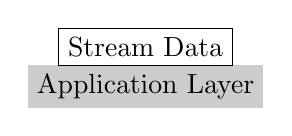
\begin{tikzpicture}
				\node (ap) [rectangle,fill=black!20] {Application Layer};
				\node (sd) [rectangle,draw,below of=ap,fill=white,yshift=1.5cm] {Stream Data};
			\end{tikzpicture}
		};
		\draw [-latex](al) -- node [midway,fill=white] {Continuous data} (dl);
		\node (pl) [sub,below of=dl,yshift=-8cm] {
			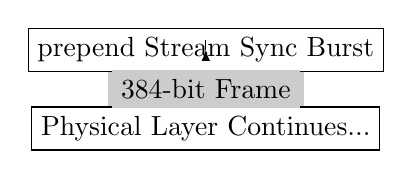
\begin{tikzpicture}
				\node (phy) [rectangle,fill=black!20] {Physical Layer};
				\node (rand) [rectangle,draw,below of=phy,fill=white,yshift=1.5cm] {randomizer};
				\node (pps) [rectangle,draw,below of=rand,fill=white,yshift=1cm] {prepend Stream Sync Burst};
				\node (plc) [rectangle,draw,below of=pps,fill=white] {Physical Layer Continues...};
				\draw [-latex](rand) -- (pps);
				\draw [-latex](pps) -- node [midway,fill=black!20] {384-bit Frame} (plc);
			\end{tikzpicture}
		};
		\draw [-latex](dl) -- node [midway,fill=white] {368 Type 4 bits} (pl);
	\end{tikzpicture}
	\caption{Stream Frame Construction}
\end{figure}

\subsection{Stream Superframes}

Stream Frames are grouped into Stream Superframes, which is the group of 6 frames that contain everything needed to rebuild the original LSF packet, so that the user who starts listening in the middle of a stream (late-joiner) is eventually able to reconstruct the LSF message and understand how to receive the in-progress stream.

\begin{figure}[H]
	\centering
	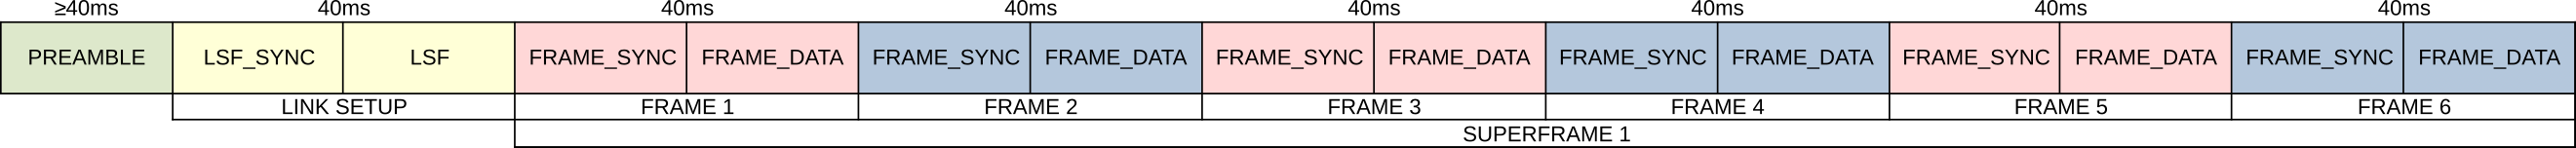
\includegraphics[width=\linewidth]{img/M17_stream}
	\caption{Stream Superframes}
	\label{fig:m17stream}
\end{figure}

\section{Packet Mode}

In Packet Mode, a Single Packet with up to 798 bytes of Application Packet Data along with an appended two byte CRC may be sent over the physical layer during one Transmission.

\begin{table}[H]
	\centering
	\begin{tblr}{
		colspec={lX},
		}
		\hline
		Bytes & Meaning \\
		\hline
		1..798 & Application Packet Data \\
		2 & CRC \\
		\hline[2px]
	\end{tblr}
	\caption{Single Packet}
\end{table}

The CRC used here is the same as described in LSF CRC.

Packet Mode shall always start with an LSF that has the LSF TYPE Packet/Stream indicator bit set to 0 (Packet Mode). Following the LSF, one to 32 Packet Frames may be sent.

Packet Mode achieves a base throughput of 5 kbps, a net throughput of approximately 4.7 kbps for the largest data payload, and over 3 kbps for 100- byte payloads. Net throughput takes into account preamble and link setup overhead.

\begin{table}[H]
	\centering
	\begin{tblr}{
			colspec={|c|X[c]|X[c]|X[c]|X[c]|[dashed]c|[dashed]X[c]|X[c]|c|},
			rows={m},
			hlines,
		}
		PREAMBLE & LSF Sync Burst & LSF Frame & Packet Sync Burst & Packet Frame & ••• & Packet Sync Burst & Packet Frame & EoT \\
	\end{tblr}
	\caption{Packet Mode}
\end{table}

\subsection{Packet Frames}

Packet Frames contain Packet Contents after ECC/FEC is applied.

\paragraph{Packet Contents}

\begin{table}[H]
	\centering
	\begin{tblr}{
		colspec={lX},
		}
		\hline
		Bits & Meaning \\
		\hline
		0..199 & 200-bit chunk of Single Packet \\
		1 & End of Frame (EOF) indicator \\
		5 & Packet Frame/Byte Counter \\
		\hline[2px]
	\end{tblr}
	\caption{Packet Contents}
\end{table}

Total: 206 Type 1 bits

The metadata field contains the 1-bit End of Frame (EOF) indicator, and the 5-bit Packet Frame/Byte Counter.

Each Packet Frame Content payload contains up to a 25-byte chunk of the Single Packet. The 25-byte chunks start with the first byte of the Application Packet data, and finally end with the 2 CRC bytes. If fewer than 25 bytes are able to be extracted from the Single Packet (i.e.~for the last Packet Frame), the Single Packet chunk is padded with undefined bytes to reach 25 bytes total. This results in a minimum of one to a maximum of 32 Packet Frames per Transmission. The Packet Frame Counter is reset to zero at the start of Packet Mode.

For each Packet Frame where there is at least 1 byte remaining in the Single Packet after removing a 25-byte chunk, the EOF metadata bit is set to zero, the Packet Frame Counter value is inserted into the Packet Frame/Byte Counter metadata field, and the Packet Frame Counter is incremented.

When there are no bytes remaining in the Single Packet after removing a 25-byte (or less) chunk, the EOF metadata bit is set to one, the Packet Byte Counter is set to the number of valid bytes extracted in the last chunk (1 to 25), i nserted into the Packet Frame/Byte Counter metadata field, and Packet Mode is ended.

\begin{table}[H]
	\centering
	\begin{tblr}{
		colspec={lX},
		}
		\hline
		Bits & Meaning \\
		\hline
		0 & Set to 0, Not end of frame \\
		1..5 & Frame number, 0..31 \\
		\hline[2px]
	\end{tblr}
	\caption{Metadata Field with EOF = 0}
\end{table}

\begin{table}[H]
	\centering
	\begin{tblr}{
		colspec={lX},
		}
		\hline
		Bits & Meaning \\
		\hline
		0 & Set to 1, End of frame \\
		1..5 & Number of bytes in frame, 1..25 \\
		\hline[2px]
	\end{tblr}
	\caption{Metadata Field with EOF = 1}
\end{table}

\paragraph{Packet Contents ECC/FEC}

The 206 Type 1 bits of the Packet Contents along with 4 flush bits are convolutionally coded using a rate 1/2 coder with constraint K=5. 210 bits total are encoded resulting in 410 Type 2 bits.

These bits are $P_3$ punctured to generate 368 Type 3 bits.

Interleaving the Type 3 bits produces 368 Type 4 bits that are ready to be passed to the Physical Layer.

Within the Physical Layer, the 368 Type 4 bits are randomized and combined with the 16-bit Packet Sync Burst, which results in a complete frame of 384 bits (384 bits / 9600bps = 40 ms).

\begin{figure}[H]
	\centering
	\begin{tikzpicture}[node distance=2cm]
		\tikzstyle{sub} = [draw,rectangle,fill=black!20]
		\node (dl) [sub] {
			\begin{tikzpicture}
				\node (dll) [rectangle,fill=black!20] {Data Link Layer};
				\node (ch200) [rectangle,draw,below of=dl,fill=white,yshift=1.5cm] {chunk 200 bits};
				\node (addm) [rectangle,draw,below of=ch200,fill=white,yshift=1cm] {add metadata};
				\node (add4) [rectangle,draw,below of=addm,fill=white] {add 4 flush bits};
				\node (conv) [rectangle,draw,below of=add4,fill=white,yshift=1cm] {convolutional encoder};
				\node (p3) [rectangle,draw,below of=conv,fill=white] {$P_3$ puncturer};
				\node (int) [rectangle,draw,below of=p3,fill=white] {interleaver};
				\draw [-latex](ch200) -- (addm);
				\draw [-latex](addm) -- node [midway,fill=black!20] {206 Type 1 bits} (add4);
				\draw [-latex](add4) -- (conv);
				\draw [-latex](conv) -- node [midway,fill=black!20] {420 Type 2 bits} (p3);
				\draw [-latex](p3) -- node [midway,fill=black!20] {368 Type 3 bits} (int);
			\end{tikzpicture}
		};
		\node (al) [sub,above of=dl,yshift=4cm] {
			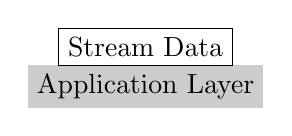
\begin{tikzpicture}
				\node (ap) [rectangle,fill=black!20] {Application Layer};
				\node (sd) [rectangle,draw,below of=ap,fill=white,yshift=1.5cm] {Stream Data};
			\end{tikzpicture}
		};
		\draw [-latex](al) -- (dl);
		\node (pl) [sub,below of=dl,yshift=-6cm] {
			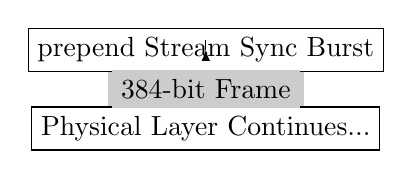
\begin{tikzpicture}
				\node (phy) [rectangle,fill=black!20] {Physical Layer};
				\node (rand) [rectangle,draw,below of=phy,fill=white,yshift=1.5cm] {randomizer};
				\node (pps) [rectangle,draw,below of=rand,fill=white,yshift=1cm] {prepend Stream Sync Burst};
				\node (plc) [rectangle,draw,below of=pps,fill=white] {Physical Layer Continues...};
				\draw [-latex](rand) -- (pps);
				\draw [-latex](pps) -- node [midway,fill=black!20] {384-bit Frame} (plc);
			\end{tikzpicture}
		};
		\draw [-latex](dl) -- node [midway,fill=white] {368 Type 4 bits} (pl);
	\end{tikzpicture};
	\caption{Packet Frame Construction}
\end{figure}

\subsection{Packet Superframes}

A Packet Superframe consists of up to the 32 Packet Frames used to reconstruct the original Single Packet.

\section{BERT Mode}

BERT mode is a standardized, interoperable mode for bit error rate testing. The preamble is sent, followed by an indefinite sequence of BERT frames. Notably, an LSF is not sent in BERT mode.

The primary purpose of defining a bit error rate testing standard for M17 is to enhance interoperability testing across M17 hardware and software implementations, and to aid in the configuration and tuning of ad hoc communications equipment common in amateur radio.

\begin{table}[H]
	\centering
	\begin{tblr}{
			colspec={|c|X[c]|X[c]|[dashed]c|[dashed]X[c]|X[c]|c|},
			rows={m},
			hlines,
		}
		PREAMBLE & BERT Sync Burst & BERT Frame  & ••• & BERT Sync Burst & BERT Frame & EoT \\
	\end{tblr}
	\caption{Packet Mode}
\end{table}

\subsection{BERT Frames}

BERT Frames contain BERT Contents after ECC/FEC is applied.

\paragraph{BERT Contents}

The BERT Contents consists of 197 bits from a \href{https://en.wikipedia.org/wiki/Pseudorandom_binary_sequence}{PRBS9} generator. This is 24 bytes and 5 bits of data. The next BERT Contents starts with the 198th bit from the PRBS9 generator. The same generator is used for each subsequent BERT Contents without being reset. The number of bits pulled from the generator, 197, is a prime number. This will produce a reasonably large number of unique frames even with a PRBS generator with a relatively short period.

See the Appendix for BERT generation and reception details.

\begin{table}[H]
	\centering
	\begin{tblr}{
		colspec={lX},
		}
		\hline
		Bits & Meaning \\
		\hline
		0-196 & BERT PRBS9 Payload \\
		\hline[2px]
	\end{tblr}
	\caption{BERT Contents}
\end{table}

Total: 197 Type 1 bits

\paragraph{BERT Contents ECC/FEC}

The 197 Type 1 bits of the Packet Contents along with 4 flush bits are convolutionally coded using a rate 1/2 coder with constraint K=5. 201 bits total are encoded resulting in 402 Type 2 bits.

These bits are $P_2$ punctured to generate 368 Type 3 bits.

Interleaving the Type 3 bits produces 368 Type 4 bits that are ready to be passed to the Physical Layer.

This provides the same error ECC/FEC used for Stream Frames.

Within the Physical Layer, the 368 Type 4 bits are randomized and combined with the 16-bit BERT Sync Burst, which results in a complete frame of 384 bits (384 bits / 9600bps = 40 ms).

\begin{figure}[H]
	\centering
	\begin{tikzpicture}[node distance=2cm]
		\tikzstyle{sub} = [draw,rectangle,fill=black!20]
		\node (dl) [sub] {
			\begin{tikzpicture}
				\node (dll) [rectangle,fill=black!20] {Data Link Layer};
				\node (bp) [rectangle,draw,below of=dl,fill=white,yshift=1.5cm] {BERT PRBS9 Data};
				\node (ch197) [rectangle,draw,below of=bp,fill=white,yshift=1cm] {chunk 197 bits};
				\node (add4) [rectangle,draw,below of=addm,fill=white] {add 4 flush bits};
				\node (conv) [rectangle,draw,below of=add4,fill=white,yshift=1cm] {convolutional encoder};
				\node (p2) [rectangle,draw,below of=conv,fill=white] {$P_2$ puncturer};
				\node (int) [rectangle,draw,below of=p2,fill=white] {interleaver};
				\draw [-latex](bp) -- (ch197);
				\draw [-latex](ch197) -- node [midway,fill=black!20] {197 Type 1 bits} (add4);
				\draw [-latex](add4) -- (conv);
				\draw [-latex](conv) -- node [midway,fill=black!20] {402 Type 2 bits} (p2);
				\draw [-latex](p2) -- node [midway,fill=black!20] {368 Type 3 bits} (int);
			\end{tikzpicture}
		};
		\node (pl) [sub,below of=dl,yshift=-6cm] {
			\begin{tikzpicture}
				\node (phy) [rectangle,fill=black!20] {Physical Layer};
				\node (rand) [rectangle,draw,below of=phy,fill=white,yshift=1.5cm] {randomizer};
				\node (ppb) [rectangle,draw,below of=rand,fill=white,yshift=1cm] {prepend BERT Sync Burst};
				\node (plc) [rectangle,draw,below of=pps,fill=white] {Physical Layer Continues...};
				\draw [-latex](rand) -- (ppb);
				\draw [-latex](ppb) -- node [midway,fill=black!20] {384-bit Frame} (plc);
			\end{tikzpicture}
		};
		\draw [-latex](dl) -- node [midway,fill=white] {368 Type 4 bits} (pl);
	\end{tikzpicture}
	\caption{BERT Frame Construction}
\end{figure}

\chapter{Application Layer}

\section{M17 Amateur Radio Voice Application}

This section defines the application layer parameters for an audio stream containing low bit rate speech encoded using the open source \href{http://rowetel.com/codec2.html}{Codec 2} codec. It is intended to be used over the air by amateur radio operators worldwide.
Implementation details for M17 clients, repeaters, and gateways ensure that an M17 Amateur Radio Voice Application is legal under all licensing regimes.

Definitions

\begin{itemize}
	\item
	M17 Client - an end station that transmits and receives M17 voice
	\item
	M17 Repeater - a station that receives and retransmits (repeats) M17
	voice
	\item
	M17 Gateway - a station that receives and transmits M17 voice,
	converting to and from different formats (e.g.~D-Star, DMR, EchoLink,
	etc.)
\end{itemize}

Credit to Jonathan Naylor (G4KLX) for documenting and implementing the details included here.

Data Link Layer Stream Mode is used for this application.

A Stream Mode Transmission begins with an LSF.

\subsection{LSF/LICH}

\begin{table}[H]
	\centering
	\begin{tblr}{
		colspec={lcX},
		}
		\hline
		Field & Length & Description \\
		\hline
		DST & 48 bits & Destination address \\
		SRC & 48 bits & Source address \\
		TYPE & 16 bits & Information about the incoming data stream \\
		META & 112 bits & Metadata field \\
		\hline[2px]
	\end{tblr}
	\caption{Link Setup Frame Contents}
\end{table}

\paragraph{Address fields}

Destination (DST) and source (SRC) addresses may be encoded amateur radio callsigns, or special identifiers. See the Address Encoding Appendix for details on how up to 9 characters of text can be encoded into the 6-byte address value.

The source address is always the callsign of the station transmitting, be it a client, repeater, or gateway. This is not a problem for a client, but for a repeater/gateway this raises issues about identifying the original source of a transmission. Having a repeater/gateway always use its own callsign for the source field does ensure that there are no issues with licensing authorities. To retain identification of the original source for a repeater/gateway, an extended callsign data field will be encoded in the LSF META field.

The destination address used by a client may simply be a callsign for a point to point contact, or may be one of the following special identifiers in the table below.

\begin{table}[H]
	\centering
	\begin{tblr}{
		colspec={lcX},
		}
		\hline
		Identifier & Address Value & Description \\
		\hline
		(Callsign) & varies & Destination callsign for a point to point
		contact \\
		ALL & 0xFFFFFFFFFFFF & Broadcast and any transmission is relayed to any connected reflector \\
		ECHO & 0x0000000ED87D & Enable the local echo function in a repeater/gateway \\
		INFO & 0x0000000ECDB9 & Trigger a voice and text announcement of the current linked status of the repeater/gateway \\
		UNLINK & 0x0000454F7745 & Unlink from a reflector and trigger an INFO	response \\
		(Reflector Name) & varies & Link to a reflector and trigger an INFO response (if valid and not already linked) \\
		\hline[2pt]
	\end{tblr}
	\caption{Client destination address}
\end{table}

The destination address of locally repeated radio transmission retains its original destination address, and the originator's callsign is encoded in the extended callsign data. For other transmissions, one of the following special identifiers may be used.

\begin{table}[H]
	\centering
	\begin{tblr}{
		colspec={lcX},
		}
		\hline
		Identifier & Address Value & Description \\
		\hline
		(Callsign) & varies & Destination callsign for a locally repeated radio transmission \\
		ALL & 0xFFFFFFFFFFFF & All transmitted reflector traffic, originator's callsign and the currently linked reflector are encoded in the extended callsign data \\
		ECHO & 0x0000000ED87D & Reply of the built-in echo function, originator's callsign is encoded in the extended callsign data \\
		INFO & 0x0000000ECDB9 & Voice and text announcement of the current linked status of the repeater/gateway \\
		\hline[2pt]
	\end{tblr}
	\caption{Repeater/gateway destination address}
\end{table}

\paragraph{TYPE field}

The TYPE field contains information about the frames to follow LSF.

\begin{table}[H]
	\centering
	\begin{tblr}{
		colspec={lX},
		}
		\hline
		Bits & Meaning \\
		\hline
		0 & Packet/Stream indicator \\
		& 1 = Stream Mode \\
		\hline
		1..2 & Data type indicator \\
		& $10_2$ = Voice only (3200 bps) \\
		\hline
		3..4 & Encryption type \\
		& $00_2$ = None \\
		& $01_2$ = Scrambling \\
		& $10_2$ = AES \\
		\hline
		5..6 & Encryption subtype \\
		\hline
		7..10 & Channel Access Number (CAN) \\
		\hline
		11..15 & Reserved (don't care) \\
		\hline[2px]
	\end{tblr}
	\caption{M17 Voice LSF TYPE definition}
\end{table}

This application requires Stream Mode.

The Voice only Data type indicator specifies voice data encoded at 3200 bps using Codec 2.

\subsection{Encryption Types}

Encryption is \textbf{optional}. The use of it may be restricted within
some radio services and countries, and should only be used if legally
permissible.

\paragraph{Null Encryption}

Encryption type = $00_2$

When no encryption is used, the 14-byte (112-bit) META field of the LSF and corresponding LICH of the stream can be used for transmitting relatively small amounts of extended data without affecting the bandwidth available for the audio. The full 14 bytes of META extended data is potentially decodable every six stream frames, at a 240 ms update rate. The extended data is transmitted in a simple round robin manner, with the only exception being GPS data which should be transmitted as soon as possible after the GPS data is received from its source.

The ``Encryption SubType'' bits in the Stream Type field indicate what extended data is stored in the META field.

\begin{table}[H]
	\centering
	\begin{tblr}{
		colspec={lX},
		}
		\hline
		Encryption subtype bits & LSF META data contents \\
		\hline
		$00_2$ & Text Data \\
		$01_2$ & GNSS Position Data \\
		$10_2$ & Extended Callsign Data \\
		$11_2$ & Reserved \\
		\hline[2px]
	\end{tblr}
	\caption{Null encryption subtype bits}
\end{table}

\paragraph{Text Data}

The first byte of the Text Data is a Control Byte. To maintain backward compatibility, a Control Byte of 0x00 indicates that no Text Data is included.

Up to four Text Data blocks compose a complete message with a maximum length of 52 bytes. Each block may contain up to 13 bytes of UTF-8 encoded text, and is padded with space characters to fill any unused space at the end of the last used Text Data block.

The Control Byte is split into two 4-bit fields. The most significant four bits are a bit map of the message length indicating how many Text Data blocks are required for a complete message. There is one bit per used Text Data block, with $0001_2$ used for one block, $0011_2$ for the two, $0111_2$ for three, and $1111_2$ for four.

The least significant four bits indicate which of the Text Data blocks this text corresponds to. It is $0001_2$ for the first, $0010_2$ for the second, $0100_2$ for the third, and $1000_2$ for the fourth. Any received Control Byte is OR-ed together by the receiving station, and once the most significant and least significant four bits are the same, a complete message has been received.

It is up to the receiver to decide how to display this message. It may choose to wait for all of the Text Data to be received, or display the parts as they are received. It is not expected that the data in the text field changes during the course of a transmission.

\paragraph{GNSS Data}

Unlike Text and Extended Callsign Data, GNSS data is expected to be dynamic during the course of a transmission and to be transmitted quickly after the GNSS data becomes available. To stop the LSF/LICH data stream from being overrun with GNSS data relative to other data types, a throttle on the amount of GNSS data transmitted is needed. It is recommended that GNSS data be sent at an update rate no faster than once every five seconds.

The GNSS data fits within one 14-byte META field, which equates to six audio frames, and takes 240ms to transmit. This is a simple format of the GNSS data which does not require too much work to convert into, and provides enough flexibility for most cases. This has been tested on-air and successfully gated to APRS-IS, showing a location very close to the position reported by the GPS receiver.

GNSS Position Data stores the 112 bit META field as follows:

\begin{table}[H]
	\begin{small}
		\begin{longtable}[]{@{}
				>{\raggedright\arraybackslash}p{(\columnwidth - 4\tabcolsep) * \real{0.1165}}
				>{\raggedright\arraybackslash}p{(\columnwidth - 4\tabcolsep) * \real{0.1650}}
				>{\raggedright\arraybackslash}p{(\columnwidth - 4\tabcolsep) * \real{0.7184}}@{}}
			\toprule
			\begin{minipage}[b]{\linewidth}\raggedright
				Size in bits
			\end{minipage} & \begin{minipage}[b]{\linewidth}\raggedright
				Format
			\end{minipage} & \begin{minipage}[b]{\linewidth}\raggedright
				Contents
			\end{minipage} \\
			\midrule
			\endhead
			8 & unsigned integer & Data Source \\
			& & Used to modify the message added to the APRS message sent to
			APRS-IS \\
			& & 0x00 : M17 Client \\
			& & 0x01 : OpenRTX \\
			& & 0x02..0xFE : reserved \\
			& & 0xFF : other data source \\
			\midrule
			8 & unsigned integer & Station Type \\
			& & Translated into suitable APRS symbols when gated to APRS-IS \\
			& & 0x00 : Fixed Station \\
			& & 0x01 : Mobile Station \\
			& & 0x02 : Handheld \\
			\midrule
			8 & unsigned integer & Whole number absolute value of degrees
			latitude \\
			\midrule
			16 & unsigned integer & Decimal degrees of latitude multiplied by 65535,
			MSB first \\
			\midrule
			8 & unsigned integer & Whole number absolute value of degrees
			longitude \\
			\midrule
			16 & unsigned integer & Decimal degrees of longitude multiplied by
			65535, MSB first \\
			\midrule
			8 & unsigned integer & Latitude N/S, Longitude E/W, Altitude, Speed and
			Bearing bit fields \\
			& & $xxxxxxx0_2$ North Latitude \\
			& & $xxxxxxx1_2$ South Latitude \\
			& & $xxxxxx0x_2$ East Longitude \\
			& & $xxxxxx1x_2$ West Longitude \\
			& & $xxxxx0xx_2$ Altitude data invalid \\
			& & $xxxxx1xx_2$ Altitude data valid \\
			& & $xxxx0xxx_2$ Speed and Bearing data invalid \\
			& & $xxxx1xxx_2$ Speed and Bearing data valid \\
			\midrule
			16 & unsigned integer & Altitude above sea level in feet + 1500 (if
			valid), MSB first \\
			\midrule
			16 & unsigned integer & Whole number of bearing in degrees between 0 and
			360 (if valid), MSB first \\
			\midrule
			8 & unsigned integer & Whole number of speed in miles per hour (if
			valid) \\
			\bottomrule
		\end{longtable}
	\end{small}
	\caption{GNSS Data encoding}
\end{table}

\paragraph{Extended Callsign Data}

This is only transmitted from repeaters/gateways and not from clients, who only receive and display this data. These fields should not appear over M17 Internet links as they should only be used over the air from a repeater/gateway.

The META field is split into two callsign fields. The first is always present, and the second is optional. The callsign data is encoded using the standard M17 callsign Address Encoding which takes six bytes to encode a nine character callsign. Any unused space in the META field contains 0x00 bytes. The first callsign field starts at offset zero in the META field, and the second callsign if present starts immediately after the first. There are two unused bytes at the end of the META field.

The use of these two callsign fields is as follows:

\begin{table}[H]
	\centering
	\begin{tblr}{
		colspec={lcX},
		}
		\hline
		Source & Callsign Field 1 & Callsign Field 2 \\
		\hline
		Locally Repeated RF & Originator & Unused \\
		ECHO Reply & Originator & Unused \\
		Reflector Traffic & Originator & Reflector Name \\
		\hline[2px]
	\end{tblr}
	\caption{Extended Callsign Data encoding}
\end{table}

The extended callsign data is not used under any other circumstances than the above currently.

It is not expected that the data in the extra callsign fields change during the course of a transmission.

\paragraph{Scrambling}

Encryption type = $01_2$

Scrambling is an encryption by bit inversion using a bitwise exclusive-or (XOR) operation between the bit sequence of data and a pseudorandom bit sequence.

Pseudorandom bit sequence is generated using a Fibonacci-topology Linear- Feedback Shift Register (LFSR). Three different LFSR sizes are available: 8, 16 and 24-bit. Each shift register has an associated polynomial. The polynomials are listed in Table 7. The LFSR is initialized with a seed value of the same length as the shift register. The seed value acts as an encryption key for the scrambler algorithm. Figures 16 to 18 show block diagrams of the algorithm.

\begin{table}[H]
	\centering
	\begin{tblr}{
		colspec={llXX},
		}
		\hline
		Encryption subtype & LFSR polynomial & Seed length & Sequence period \\
		\hline
		$00_2$ & $x^8 + x^6 + x^5 + x^4 + 1$ & 8 bits & 255 \\
		$01_2$ & $x^{16} + x^{15} + x^{13} + x^4 + 1$ & 16 bits & 65,535 \\
		$10_2$ & $x^{24} + x^{23} + x^{22} + x^{17} + 1$ & 24 bits &
		16,777,215 \\
		\hline[2px]
	\end{tblr}
	\caption{Scrambling}
\end{table}

\begin{figure}[H]
	\centering
	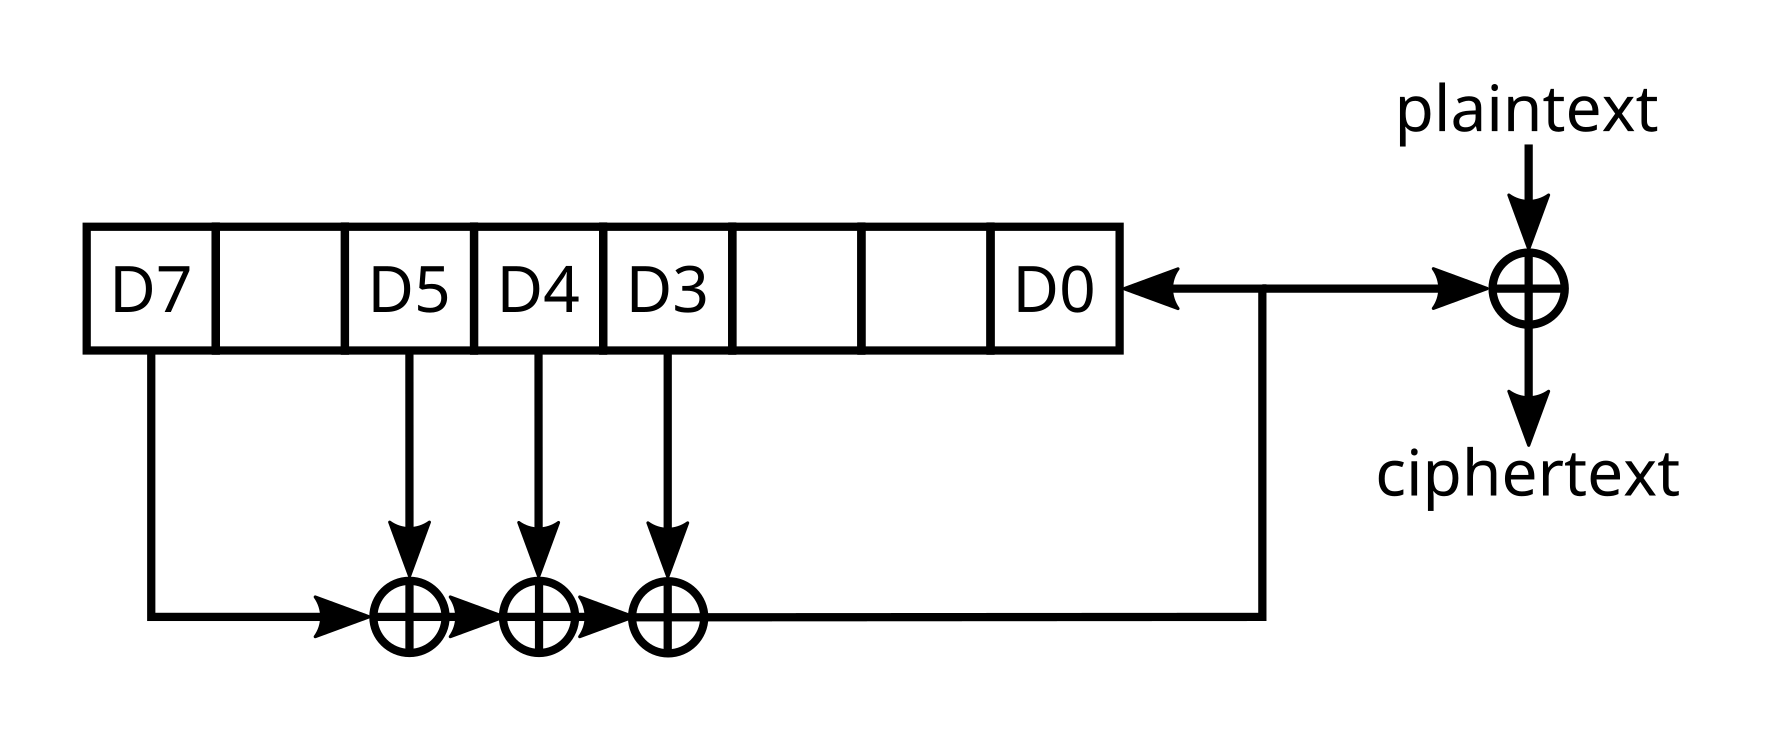
\includegraphics{img/LFSR_8}
	\caption{8-bit LFSR taps}
	\label{fig:lfsr8}
\end{figure}

\begin{figure}[H]
	\centering
	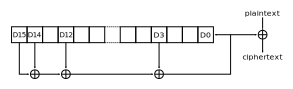
\includegraphics{img/LFSR_16}
	\caption{16-bit LFSR taps}
	\label{fig:lfsr16}
\end{figure}

\begin{figure}[H]
	\centering
	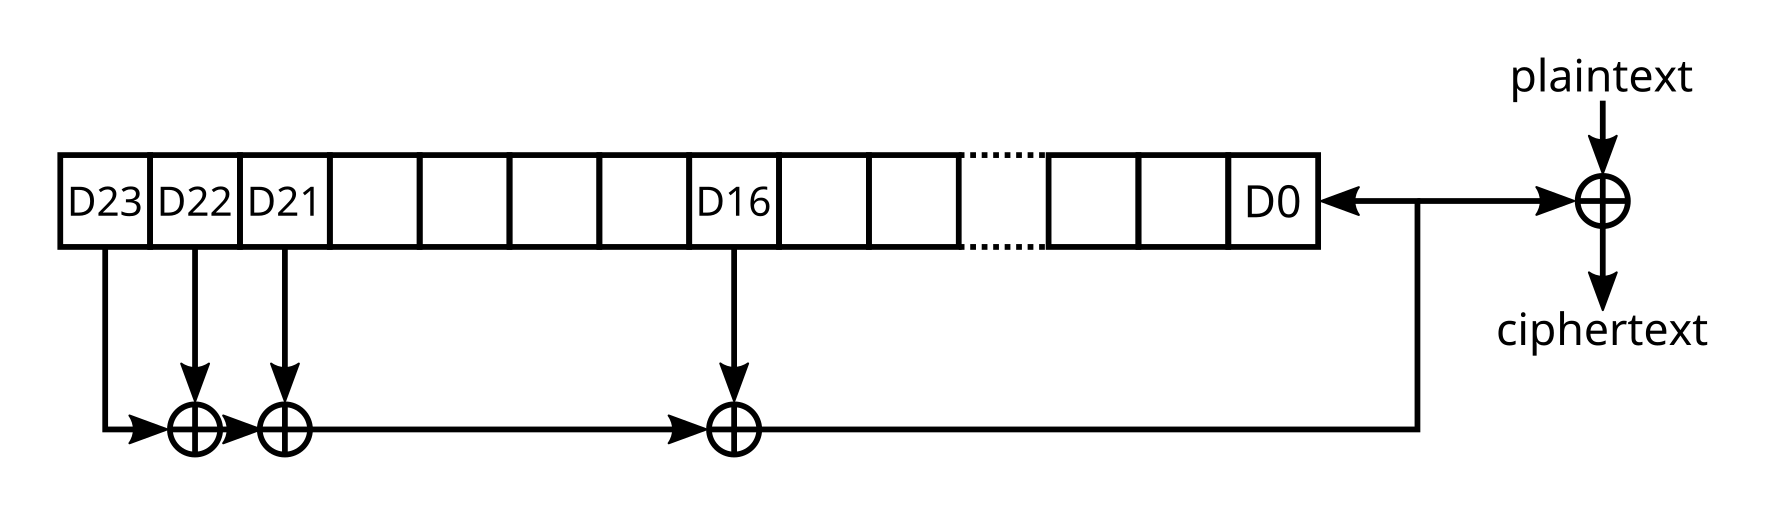
\includegraphics{img/LFSR_24}
	\caption{24-bit LFSR taps}
	\label{fig:lfsr24}
\end{figure}

\paragraph{Advanced Encryption Standard (AES)}

Encryption type = $10_2$

This method uses AES block cipher in counter (CTR) mode, with a 96-bit nonce that should never be used for more than one separate stream and a 32-bit CTR.

The 96-bit AES nonce value is extracted from the 96 most significant bits of the META field, and the remaining 16 bits of the META field form the highest 16 bits of the 32-bit counter. The FN (Frame Number) field value is then used to fill out the lower 16 bits of the counter, and always starts from 0 (zero) in a new voice stream.

The 16-bit frame number and 40 ms frames can provide for over 20 minutes of streaming without rolling over the counter.

\begin{quote}
	NOTE The effective capacity of the counter is 15 bits, as the MSB is used for transmission end signalling. At 40ms per frame, or 25 frames per second, and $2^{15}$ frames, we get $2^{15}$ frames / 25 frames per second = 1310 seconds, or almost 22 minutes.
\end{quote}

The random part of the nonce value should be generated with a hardware random number generator or any other method of generating non-repeating values.

To combat replay attacks, a 32-bit timestamp shall be embedded into the cryptographic nonce field. The field structure of the 96 bit nonce is shown in Table 9. Timestamp is 32 LSB portion of the number of seconds that elapsed since the beginning of 1970-01-01, 00:00:00 UTC, minus leap seconds (a.k.a. ``unix time'').

\paragraph{96 bit nonce field structure}

CTR\_HIGH field initializes the highest 16 bits of the CTR, with the rest of the counter being equal to the FN counter. Encryption subtypes are not applicable for this encryption scheme. All parties are assumed to know the key length used for each transmission.

\begin{table}[h]
	\centering
	\begin{tblr}{
		colspec={XXX},
		}
		\hline
		Timestamp & Random Data & CTR\_HIGH \\
		\hline
		32 & 64 & 16 \\
		\hline[2px]
	\end{tblr}
	\caption{Nonce field}
\end{table}

\begin{quote}
	WARNING In CTR mode, AES encryption is malleable. That is, an attacker can change the contents of the encrypted message without decrypting it. This means that recipients of AES-encrypted data must not trust that the data is authentic. Users who require that received messages are proven to be exactly as-sent by the sender should add application-layer authentication, such as HMAC. In the future, use of a different mode, such as Galois/Counter Mode, could alleviate this issue.
\end{quote}

\subsection{Channel Access Number (CAN)}

The Channel Access Number (CAN) is a four bit code that may be used to filter received audio, text, and GNSS data. A receiver may optionally allow reception from sources only if their transmitted CAN value matches the receiver's own specified CAN value.

\subsection{Stream Frames}

Stream Frames will contain the appropriate LICH data (described above). The Stream Contents will include the incrementing 16-bit Frame Number, and 128 bits of Codec 2 data (unencrypted or encrypted).

\section{Packet Application}

\begin{quote}
	ATTENTION This is work in progress.
\end{quote}

A single packet of up to 798 bytes of data may be sent in one transmission.

Packets are sent using Packet Mode.

A Stream Mode Transmission begins with an LSF.

Packet superframes are composed of a 1..n byte data type specifier, 0..797 bytes of payload data. The data type specifier is encoded in the same way as UTF-8. It provides efficient coding of common data types. And it can be extended to include a very large number of distinct packet data type codes.

The data type specifier can also be used as a protocol specifier. For example, the following protocol identifiers are reserved in the M17 packet spec:

\begin{table}[H]
	\centering
	\begin{tblr}{
		colspec={XX},
		}
		\hline
		Identifier & Protocol \\
		\hline
		0x00 & RAW \\
		0x01 & AX.25 \\
		0x02 & APRS \\
		0x03 & 6LoWPAN \\
		0x04 & IPv4 \\
		0x05 & SMS \\
		0x06 & Winlink \\
		\hline[2px]
	\end{tblr}
	\caption{Packet protocol identifiers}
\end{table}

The data type specifier is used to compute the CRC, along with the payload.

\chapter{IP Networking}

Digital modes are commonly networked together through linked repeaters using IP networking.

For commercial protocols like DMR, this is meant for linking metropolitan and state networks together and allows for easy interoperability between radio users. Amateur Radio uses this capability for creating global communications networks for all imaginable purposes, and makes `working the world' with an HT possible.

M17 is designed with this use in mind, and has native IP framing to support it.

In competing radio protocols, a repeater or some other RF to IP bridge is required for linking, leading to the use of hotspots (tiny simplex RF bridges).

The TR-9 and other M17 radios may support IP networking directly, such as through the ubiquitous ESP8266 chip or similar. This allows them to skip the RF link that current hotspot systems require, finally bringing to fruition the ``Amateur digital radio is just VoIP'' dystopian future we were all warned about.

\section{Standard IP Framing}

M17 over IP is big endian, consistent with other IP protocols. We have standardized on UDP port 17000, this port is recommended but not required. Later specifications may require this port.

\begin{table}[H]
	\centering
	\begin{tblr}{
		colspec={llX},
		}
		\hline
		Field & Size & Description \\
		\hline
		MAGIC & 32 bits & Magic bytes 0x4d313720 (``M17 '') \\
		StreamID (SID) & 16 bits & Random bits, changed for each PTT or stream, but consistent from frame to frame within a stream \\
		LICH & 224 bits & The meaningful contents of a LICH frame (dst, src, streamtype, META field) as defined earlier. \\
		FN & 16 bits & Frame number (exactly as would be transmitted as an RF stream frame, including the last frame indicator at (FN \& 0x8000) \\
		Payload & 128 bits & Payload (exactly as would be transmitted in an RF stream frame) \\
		CRC16 & 16 bits & CRC for the entire packet, as defined earlier CRC definition \\
		\hline[2pt]
	\end{tblr}
\end{table}

The CRC checksum must be recomputed after modification or re-assembly of the packet, such as when translating from RF to IP framing.

\section{Control Packets}

Reflectors use a few different types of control frames, identified by
their magic:

\begin{itemize}
	\item
	CONN - Connect to a reflector
	\item
	ACKN - acknowledge connection
	\item
	NACK - deny connection
	\item
	PING - keepalive for the connection from the reflector to the client
	\item
	PONG - keepalive response from the client to the reflector
	\item
	DISC - Disconnect (client-\textgreater reflector or
	reflector-\textgreater client)
\end{itemize}

\subsection{CONN}

\begin{table}[H]
	\centering
	\begin{tblr}{
		colspec={lX},
		}
		\hline
		Bytes & Purpose \\
		\hline
		0..3 & Magic - ASCII ``CONN'' \\
		4..9 & 6-byte `From' callsign including module in last character (e.g.~``A1BCD D'') encoded as per Address Encoding \\
		10 & Module to connect to - single ASCII byte A-Z \\
		\hline[2px]
	\end{tblr}
	\caption{Bytes of CONN Packet}
\end{table}

A client sends this to a reflector to initiate a connection. The reflector replies with ACKN on successful linking, or NACK on failure.

\subsection{ACKN}

\begin{table}[H]
	\centering
	\begin{tblr}{
		colspec={lX},
		}
		\hline	
		Bytes & Purpose \\
		\hline
		0..3 & Magic - ASCII ``ACKN'' \\
		\hline[2px]
	\end{tblr}
	\caption{Bytes of ACKN Packet}
\end{table}

\subsection{NACK}

\begin{table}[H]
	\centering
	\begin{tblr}{
		colspec={lX},
		}
		\hline
		Bytes & Purpose \\
		\hline
		0..3 & Magic - ASCII ``NACK'' \\
		\hline[2px]
	\end{tblr}
	\caption{Bytes of NACK Packet}
\end{table}

\subsection{PING}

\begin{table}[H]
	\centering
	\begin{tblr}{
		colspec={lX},
		}
		\hline
		Bytes & Purpose \\
		\hline
		0..3 & Magic - ASCII ``PING'' \\
		4..9 & 6-byte `From' callsign including module in last character (e.g.~``A1BCD D'') encoded as per Address Encoding \\
		\hline[2px]
	\end{tblr}
	\caption{Bytes of PING Packet}
\end{table}

\subsection{PONG}

\begin{table}[H]
	\centering
	\begin{tblr}{
			colspec={lX},
		}
		\hline
		Bytes & Purpose \\
		\hline
		0..3 & Magic - ASCII ``PONG'' \\
		4..9 & 6-byte `From' callsign including module in last character (e.g.~``A1BCD D'') encoded as per Address Encoding \\
		\hline[2px]
	\end{tblr}
	\caption{Bytes of PONG Packet}
\end{table}

\subsection{DISC}

\begin{table}[H]
	\centering
	\begin{tblr}{
		colspec={lX},
		}
		\hline
		Bytes & Purpose \\
		\hline
		0..3 & Magic - ASCII ``DISC'' \\
		4..9 & 6-byte `From' callsign including module in last character (e.g.~``A1BCD D'') encoded as per Address Encoding \\
		\hline[2px]
	\end{tblr}
	\caption{Bytes of DISC Packet}
\end{table}

\appendix

\chapter{Address Encoding}

M17 uses 48-bit (6-byte) addresses. Callsigns and special purpose
addresses are encoded into these 6 bytes in the following ways:

\begin{itemize}
	\item
	An address of \texttt{0} is invalid.
	\item
	Address values between \texttt{1} and \texttt{262143999999999} ($40^{9}-1$), contain up to 9 characters of text encoded using base-40 as described below.
	\item
	Address values between \texttt{262144000000000} ($40^{9}$) and \texttt{281474976710654} ($2^{48}-2$) are reserved for future use.
	\item
	An address of \texttt{0xFFFFFFFFFFFF} is a broadcast.
\end{itemize}

\section{Address Scheme}

\begin{table}[H]
	\centering
	\begin{tblr}{
		colspec={lllX},
		}
		\hline
		Address Range (base-16) & Category & Number of Addresses & Remarks \\
		\hline
		\texttt{0x000000000000} & INVALID & 1 & \\
		\hline
		\texttt{0x000000000001 - 0xEE6B27FFFFFF} & Unit ID & 262,143,999,999,999 & \\
		\hline
		\texttt{0xEE6B28000000 - 0xFFFFFFFFFFFE} & RESERVED & 19,330,976,710,655 & For future use \\
		\hline
		\texttt{0xFFFFFFFFFFFF} & Broadcast & 1 & Valid only for destination \\
		\hline[2pt]	
	\end{tblr}
	\caption{M17 Addresses}
\end{table}

\section{Callsign Encoding: base-40}

9 characters from an alphabet of 40 possible characters can be encoded
into 48 bits (6 bytes). The base-40 alphabet is:

\begin{table}[H]
	\centering
	\begin{tblr}{
		colspec={llX},
		}
		\hline
		Value (base-10) & Character & Note \\
		\hline
		0 & ' ' & A space, ASCII 32 (0x20). Invalid characters will be replaced
		with this. \\
		1 - 26 & `A' - `Z' & Upper case letters, ASCII 65 - 90 (0x41 - 0x5A). \\
		27 - 36 & `0' - `9' & Numerals, ASCII 48 - 57 (0x30 - 0x39). \\
		37 & `-' & Hyphen, ASCII 45 (0x2D). \\
		38 & `/' & Forward Slash, ASCII 47 (0x2F). \\
		39 & `.' & Dot, ASCII 46 (0x2E). \\
		\hline[2px]
	\end{tblr}
	\caption{M17 Callsign Alphabet}
\end{table}

When computing the base-40 value of the callsign, the left most character of the callsign is the least significant value. Callsigns must be left justified. Leading spaces are not permitted.

After the base-40 value is calculated, the final 6-byte address is the big endian encoded (most significant byte first) representation of the base-40 value.

For example, for the callsign AB1CD, the base-40 representation would be DC1BA, and would be calculated as:

(`D': $4 \times 40^4$) + (`C': $3 \times 40^3$) + (`1': $28 \times 40^2$) + (`B': $2 \times 40^1$) + (`A': $1 \times 40^0$)

DC1BA (base-40), \texttt{0$\times$0000009fdd51} (base-16), 10476881 (base-10)

The final address encoded into the 6-byte LSF/LICH field would be \texttt{0$\times$0000009fdd51}

\section{Example Encoder}

\begin{lstlisting}[language=Python]
def encodeM17(call):
	"""Encode a text string into an M17 address value"""
	
	charMap = ' ABCDEFGHIJKLMNOPQRSTUVWXYZ0123456789-/.'
	
	# convert to upper case
	call = call.upper()
	
	# generate an assert error if more than 9 characters long
	assert len(call) <= 9, 'Error: <callsign> must be 9 characters or less'
	
	if call == 'ALL':
	# handle the special case for Broadcast
	encoded = 0xFFFFFFFFFFFF
	else:
	encoded = 0
	# loop through the characters starting from the end (right most character)
	for c in call[::-1]:
	# find the position of the character in the map
	value = charMap.find(c)
	
	# if value < 0, the character was not found
	# invalid characters are forced to 0
	if value < 0:
	value = 0
	
	# shift the current value by one base-40 character (40 decimal)
	# and add the current value
	encoded = encoded*40 + value
	
	return encoded
\end{lstlisting}

\section{Example Decoder}

\begin{lstlisting}[language=Python]
def decodeM17(encoded):
	"""Decode an M17 address value to a text string"""
	
	charMap = ' ABCDEFGHIJKLMNOPQRSTUVWXYZ0123456789-/.'
	
	# check for unique values
	if encoded == 0xFFFFFFFFFFFF:
	# BROADCAST
	call = 'ALL'
	elif encoded == 0:
	call = 'RESERVED'
	elif encoded >= 0xEE6B28000000:
	call = 'RESERVED'
	else:
	call = ''
	while (encoded > 0):
	call = call + charMap[encoded % 40]
	encoded = encoded // 40
	
	return call
\end{lstlisting}

\section{Why base-40?}

\subsection{Callsign Formats}

The \href{https://www.itu.int/}{International Telecommunication Union (ITU)} coordinates radio callsign formats worldwide, with format details specified in ITU \href{https://www.itu.int/pub/R-REG-RR/en}{Radio Regulations} Articles 19.67 through 19.69. A very extensive \href{https://en.wikipedia.org/wiki/Amateur_radio_call_signs}{Wikipedia
entry for Amateur Radio Call Signs} includes implementation details on callsign use around the world.

From the ITU Articles, the longest standard callsign may consist of up to seven characters, with longer temporary special occasion callsigns allowed. The allowed callsign characters, or ``callsign alphabet'', are the 26 letters of the English alphabet (`A' through `Z') and the ten digits (`0' through `9').

\paragraph{Secondary Operating Suffixes}

Secondary operating suffixes are often added to callsign to indicate temporary changes of status, such as ``AB1CD/M'' for a mobile station, or ``AB1CD/AE'' to signify the station has additional operating privileges, etc. The `/' character will be included in callsign alphabet.

\paragraph{Bits per Characters}

The minimum number of allowed callsign characters in the callsign alphabet is 37 (`A' through `Z', `0' through `9', and `/'). The following table shows how many bytes are required to encoded a callsign using an alphabet size of 37.

\begin{table}[H]
	\centering
	\begin{tblr}{
		colspec={llX},
		}
		\hline
		Callsign Characters & Bits & Bytes \\
		\hline
		7 & \(log_2(37^7)=36.47\) & 5 \\
		8 & \(log_2(37^8)=41.67\) & 6 \\
		9 & \(log_2(37^9)=46.89\) & 6 \\
		10 & \(log_2(37^{10})=52.09\) & 7 \\
		11 & \(log_2(37^{11})=57.30\) & 8 \\
		12 & \(log_2(37^{12})=62.51\) & 8 \\
		13 & \(log_2(37^{13})=67.72\) & 9 \\
		\hline[2px]
	\end{tblr}
	\caption{Storage required for number of callsign characters}
\end{table}

Of these, 9 characters into 6 bytes, or 12 characters into 8 bytes are
the most efficient. Given that 9 callsign characters and 6 bytes should
be suitable for the majority of use cases, can the callsign alphabet be
increased without using more than 6 bytes?

\paragraph{Alphabet Size vs.~Bytes}

The following table shows how many bytes are required to encode a 9 character callsign using callsign alphabet sizes of 37 through 41.

\begin{table}[H]
	\centering
	\begin{tblr}{
		colspec={llX},
		}
		\hline
		Alphabet Size & Bits & Bytes \\
		\hline
		37 & \(log_2(37^9)=46.89\) & 6 \\
		38 & \(log_2(38^9)=47.23\) & 6 \\
		39 & \(log_2(39^9)=47.57\) & 6 \\
		40 & \(log_2(40^9)=47.90\) & 6 \\
		41 & \(log_2(41^9)=48.22\) & 7 \\
		\hline[2px]
	\end{tblr}
	\caption{Storage required for alphabet size}
\end{table}

The largest callsign alphabet size able to encode 9 characters into 6
bytes is 40. This means the minimal callsign alphabet of 37 can be
extended with three additional characters.

\subsection{Multiple Stations}

To indicate multiple stations by the same operator, the `-' character can be used. A callsign such as ``AB1CD-1'' is considered a different station than ``AB1CD-2'' or even ``AB1CD'', but it is understood that these all belong to the same operator, ``AB1CD''. The `-' character will be included in callsign alphabet.

\subsection{Fill}

A space ' ' character is included in the callsign alphabet as a fill character or as a substitute for characters that are not part of the callsign alphabet.

\subsection{Dot}

A dot `.' character is included in the callsign alphabet as \ldots{} TBD \ldots{}

\subsection{M17 base-40 Callsign Alphabet}

These final additions complete the 40 character M17 callsign alphabet as ' ' (space), `A' through `Z', `0' through `9', `-' (hyphen), `/' (forward slash), and `.' (dot).

\chapter{Randomizer Sequence}

\begin{table}[H]
	\centering
	\begin{tblr}{
		colspec={lXlX},
		}
		\hline
		Seq. number & Value & Seq. number & Value \\
		\hline
		00 & 0xD6 & 23 & 0x6E \\
		01 & 0xB5 & 24 & 0x68 \\
		02 & 0xE2 & 25 & 0x2F \\
		03 & 0x30 & 26 & 0x35 \\
		04 & 0x82 & 27 & 0xDA \\
		05 & 0xFF & 28 & 0x14 \\
		06 & 0x84 & 29 & 0xEA \\
		07 & 0x62 & 30 & 0xCD \\
		08 & 0xBA & 31 & 0x76 \\
		09 & 0x4E & 32 & 0x19 \\
		10 & 0x96 & 33 & 0x8D \\
		11 & 0x90 & 34 & 0xD5 \\
		12 & 0xD8 & 35 & 0x80 \\
		13 & 0x98 & 36 & 0xD1 \\
		14 & 0xDD & 37 & 0x33 \\
		15 & 0x5D & 38 & 0x87 \\
		16 & 0x0C & 39 & 0x13 \\
		17 & 0xC8 & 40 & 0x57 \\
		18 & 0x52 & 41 & 0x18 \\
		19 & 0x43 & 42 & 0x2D \\
		20 & 0x91 & 43 & 0x29 \\
		21 & 0x1D & 44 & 0x78 \\
		22 & 0xF8 & 45 & 0xC3 \\
		\hline[2px]
	\end{tblr}
	\caption{Randomizer values}
\end{table}

\chapter{Convolutional Encoder}

The convolutional code shall encode the input bit sequence after
appending 4 tail bits at the end of the sequence. Rate of the coder is
R=½ with constraint length K=5. The encoder diagram and generating
polynomials are shown below.

\begin{align*}
	G_1(D) =& 1 + D^3 + D^4 \\
	G_2(D) =& 1+ D + D^2 + D^4
\end{align*}

The output from the encoder must be read alternately.

\begin{figure}[H]
	\centering
	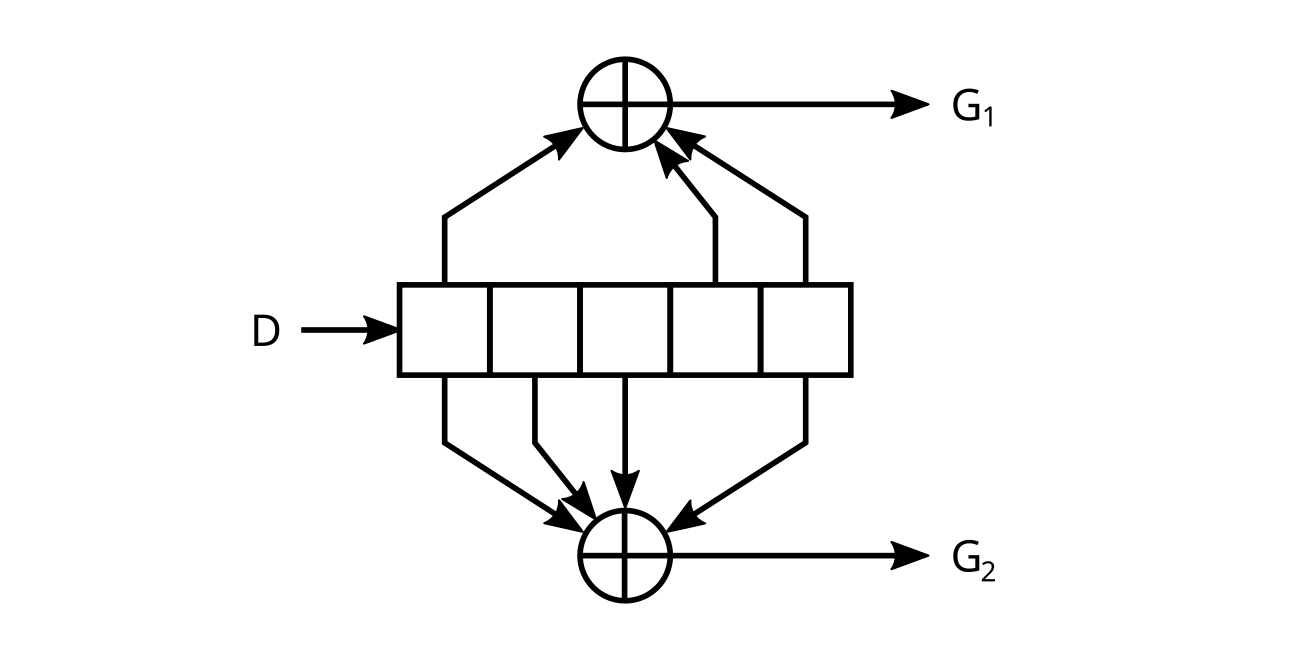
\includegraphics{img/convolutional}
	\caption{Convolutional encoder}
	\label{fig:convolutional}
\end{figure}

\chapter{Golay Encoder}

The extended Golay(24,12) encoder uses generating polynomial \emph{g(x)} given below to generate the 11 check bits. The check bits and an additional parity bit are appended to the 12 bit data, resulting in a 24 bit codeword. The resulting code is systematic, meaning that the input data (message) is embedded in the codeword.

$g(x) = x^{11} + x^{10} + x^6 + x^5 + x^4 + x^2 + 1$

This is equivalent to 0xC75 in hexadecimal notation. Both the generating matrix $G$ and parity check matrix $H$ are shown below.

\begin{align}
	G = [I_{12}|P] = \left[
	\begin{array}{cr}
		I_{12} \begin{matrix} 
			1&1&0&0&0&1&1&1&0&1&0&1 \\
			0&1&1&0&0&0&1&1&1&0&1&1 \\
			1&1&1&1&0&1&1&0&1&0&0&0 \\
			0&1&1&1&1&0&1&1&0&1&0&0 \\
			0&0&1&1&1&1&0&1&1&0&1&0 \\
			1&1&0&1&1&0&0&1&1&0&0&1 \\
			0&1&1&0&1&1&0&0&1&1&0&1 \\
			0&0&1&1&0&1&1&0&0&1&1&1 \\
			1&1&0&1&1&1&0&0&0&1&1&0 \\
			1&0&1&0&1&0&0&1&0&1&1&1 \\
			1&0&0&1&0&0&1&1&1&1&1&0 \\
			1&0&0&0&1&1&1&0&1&0&1&1
		\end{matrix}
	\end{array}
	\right]
\end{align}
\begin{align}
	H = [P^T|I_{12}] = \left[
	\begin{array}{cr}
		\begin{matrix}
			1&0&1&0&0&1&0&0&1&1&1&1 \\
			1&1&1&1&0&1&1&0&1&0&0&0 \\
			0&1&1&1&1&0&1&1&0&1&0&0 \\
			0&0&1&1&1&1&0&1&1&0&1&0 \\
			0&0&0&1&1&1&1&0&1&1&0&1 \\
			1&0&1&0&1&0&1&1&1&0&0&1 \\
			1&1&1&1&0&0&0&1&0&0&1&1 \\
			1&1&0&1&1&1&0&0&0&1&1&0 \\
			0&1&1&0&1&1&1&0&0&0&1&1 \\
			1&0&0&1&0&0&1&1&1&1&1&0 \\
			0&1&0&0&1&0&0&1&1&1&1&1 \\
			1&1&0&0&0&1&1&1&0&1&0&1
		\end{matrix} I_{12}
	\end{array}
	\right]
\end{align}

The output of the Golay encoder is shown in the table below.

\begin{table}[H]
	\centering
	\begin{tblr}{
		colspec={lllX},
		}
		\hline
		Field & Data & Check bits & Parity \\
		\hline
		Position & 23..12 & 11..1 & 0 (LSB) \\
		Length & 12 & 11 & 1 \\
		\hline
	\end{tblr}
	\caption{Golay encoder details}
\end{table}

Four of these 24-bit blocks are used to reconstruct the LSF.

Sample MATLAB/Octave code snippet for generating $G$ and $H$ matrices is shown below.

\begin{lstlisting}[language=Matlab]
	P = hex2poly('0xC75');
	[H,G] = cyclgen(23, P);
	
	G_P = G(1:12, 1:11);
	I_K = eye(12);
	G = [I_K G_P P.'];
	H = [transpose([G_P P.']) I_K];
\end{lstlisting}

\chapter{Code Puncturing}

Removing some of the bits from the convolutional coder's output is
called code puncturing. The nominal coding rate of the encoder used in
M17 is ½. This means the encoder outputs two bits for every bit of the
input data stream. To get other (higher) coding rates, a puncturing
scheme has to be used.

Two different puncturing schemes are used in M17 stream mode:

\begin{enumerate}
	\def\labelenumi{\arabic{enumi}.}
	\item
	$P_1$ leaving 46 from 61 encoded bits
	\item
	$P_2$ leaving 11 from 12 encoded bits
\end{enumerate}

Scheme $P_1$ is used for the \emph{link setup frame}, taking 488 bits of encoded data and selecting 368 bits. The $gcd(368, 488)$ is 8 which, when used to divide, leaves 46 and 61 bits. However, a full puncture pattern requires the puncturing matrix entries count to be divisible by the number of encoding polynomials. For this case a partial puncture matrix is used. It has 61 entries with 46 of them being ones and shall be used 8 times, repeatedly. The construction of the partial puncturing pattern $P_1$ is as follows:

\begin{align}
	M = & \begin{bmatrix}
		1 & 0 & 1 & 1
	\end{bmatrix} \\
	P_{1} = & \begin{bmatrix}
		1 & M_{1} & \cdots & M_{15}
	\end{bmatrix}
\end{align}

In which $M$ is a standard 2/3 rate puncture matrix and is used 15 times, along with a leading $1$ to form $P_1$, an array of length 61.

The first pass of the partial puncturer discards $G_1$ bits only, second pass discards $G_2$, third - $G_1$ again, and so on. This ensures that both bits are punctured out evenly.

Scheme $P_2$ is for frames (excluding LICH chunks, which are coded differently). This takes 296 encoded bits and selects 272 of them. Every 12th bit is being punctured out, leaving 272 bits. The full matrix shall have 12 entries with 11 being ones.

The puncturing scheme $P_2$ is defined by its partial puncturing matrix:

\begin{align}
	P_2 = & \begin{bmatrix}
		1 & 1 & 1 & 1 & 1 & 1 \\
		1 & 1 & 1 & 1 & 1 & 0
	\end{bmatrix}
\end{align}

The linearized representations are:

\begin{verbatim}
	P1 = [1, 1, 0, 1, 1, 1, 0, 1, 1, 1, 0, 1, 1, 1, 0, 1, 1, 1, 0, 1, 1,
	      1, 0, 1, 1, 1, 0, 1, 1, 1, 0, 1, 1, 1, 0, 1, 1, 1, 0, 1, 1, 1,
	      0, 1, 1, 1, 0, 1, 1, 1, 0, 1, 1, 1, 0, 1, 1, 1, 0, 1, 1]
	
	P2 = [1, 1, 1, 1, 1, 1, 1, 1, 1, 1, 1, 0]
\end{verbatim}

One additional puncturing scheme $P_3$ is used in the packet mode. The puncturing scheme is defined by its puncturing matrix:

\begin{align}
	P_3 = & \begin{bmatrix}
		1 & 1 & 1 & 1 \\
		1 & 1 & 1 & 0
	\end{bmatrix}
\end{align}

The linearized representation is:

\begin{verbatim}
	P3 = [1, 1, 1, 1, 1, 1, 1, 0]
\end{verbatim}

\chapter{Interleaving}

For interleaving a Quadratic Permutation Polynomial (QPP) is used. The polynomial 

$\pi(x)=(45x+92x^2)\mod 368$ 

is used for a 368 bit interleaving pattern QPP.

\begin{longtable}[]{@{}
		>{\raggedright\arraybackslash}p{(\columnwidth - 14\tabcolsep) * \real{0.1196}}
		>{\raggedright\arraybackslash}p{(\columnwidth - 14\tabcolsep) * \real{0.1304}}
		>{\raggedright\arraybackslash}p{(\columnwidth - 14\tabcolsep) * \real{0.1196}}
		>{\raggedright\arraybackslash}p{(\columnwidth - 14\tabcolsep) * \real{0.1304}}
		>{\raggedright\arraybackslash}p{(\columnwidth - 14\tabcolsep) * \real{0.1196}}
		>{\raggedright\arraybackslash}p{(\columnwidth - 14\tabcolsep) * \real{0.1304}}
		>{\raggedright\arraybackslash}p{(\columnwidth - 14\tabcolsep) * \real{0.1196}}
		>{\raggedright\arraybackslash}p{(\columnwidth - 14\tabcolsep) * \real{0.1304}}@{}}
	\toprule
	\begin{minipage}[b]{\linewidth}\raggedright
		input index
	\end{minipage} & \begin{minipage}[b]{\linewidth}\raggedright
		output index
	\end{minipage} & \begin{minipage}[b]{\linewidth}\raggedright
		input index
	\end{minipage} & \begin{minipage}[b]{\linewidth}\raggedright
		output index
	\end{minipage} & \begin{minipage}[b]{\linewidth}\raggedright
		input index
	\end{minipage} & \begin{minipage}[b]{\linewidth}\raggedright
		output index
	\end{minipage} & \begin{minipage}[b]{\linewidth}\raggedright
		input index
	\end{minipage} & \begin{minipage}[b]{\linewidth}\raggedright
		output index
	\end{minipage} \\
	\midrule
	\endhead
	0 & 0 & 92 & 92 & 184 & 184 & 276 & 276 \\
	1 & 137 & 93 & 229 & 185 & 321 & 277 & 45 \\
	2 & 90 & 94 & 182 & 186 & 274 & 278 & 366 \\
	3 & 227 & 95 & 319 & 187 & 43 & 279 & 135 \\
	4 & 180 & 96 & 272 & 188 & 364 & 280 & 88 \\
	5 & 317 & 97 & 41 & 189 & 133 & 281 & 225 \\
	6 & 270 & 98 & 362 & 190 & 86 & 282 & 178 \\
	7 & 39 & 99 & 131 & 191 & 223 & 283 & 315 \\
	8 & 360 & 100 & 84 & 192 & 176 & 284 & 268 \\
	9 & 129 & 101 & 221 & 193 & 313 & 285 & 37 \\
	10 & 82 & 102 & 174 & 194 & 266 & 286 & 358 \\
	11 & 219 & 103 & 311 & 195 & 35 & 287 & 127 \\
	12 & 172 & 104 & 264 & 196 & 356 & 288 & 80 \\
	13 & 309 & 105 & 33 & 197 & 125 & 289 & 217 \\
	14 & 262 & 106 & 354 & 198 & 78 & 290 & 170 \\
	15 & 31 & 107 & 123 & 199 & 215 & 291 & 307 \\
	16 & 352 & 108 & 76 & 200 & 168 & 292 & 260 \\
	17 & 121 & 109 & 213 & 201 & 305 & 293 & 29 \\
	18 & 74 & 110 & 166 & 202 & 258 & 294 & 350 \\
	19 & 211 & 111 & 303 & 203 & 27 & 295 & 119 \\
	20 & 164 & 112 & 256 & 204 & 348 & 296 & 72 \\
	21 & 301 & 113 & 25 & 205 & 117 & 297 & 209 \\
	22 & 254 & 114 & 346 & 206 & 70 & 298 & 162 \\
	23 & 23 & 115 & 115 & 207 & 207 & 299 & 299 \\
	24 & 344 & 116 & 68 & 208 & 160 & 300 & 252 \\
	25 & 113 & 117 & 205 & 209 & 297 & 301 & 21 \\
	26 & 66 & 118 & 158 & 210 & 250 & 302 & 342 \\
	27 & 203 & 119 & 295 & 211 & 19 & 303 & 111 \\
	28 & 156 & 120 & 248 & 212 & 340 & 304 & 64 \\
	29 & 293 & 121 & 17 & 213 & 109 & 305 & 201 \\
	30 & 246 & 122 & 338 & 214 & 62 & 306 & 154 \\
	31 & 15 & 123 & 107 & 215 & 199 & 307 & 291 \\
	32 & 336 & 124 & 60 & 216 & 152 & 308 & 244 \\
	33 & 105 & 125 & 197 & 217 & 289 & 309 & 13 \\
	34 & 58 & 126 & 150 & 218 & 242 & 310 & 334 \\
	35 & 195 & 127 & 287 & 219 & 11 & 311 & 103 \\
	36 & 148 & 128 & 240 & 220 & 332 & 312 & 56 \\
	37 & 285 & 129 & 9 & 221 & 101 & 313 & 193 \\
	38 & 238 & 130 & 330 & 222 & 54 & 314 & 146 \\
	39 & 7 & 131 & 99 & 223 & 191 & 315 & 283 \\
	40 & 328 & 132 & 52 & 224 & 144 & 316 & 236 \\
	41 & 97 & 133 & 189 & 225 & 281 & 317 & 5 \\
	42 & 50 & 134 & 142 & 226 & 234 & 318 & 326 \\
	43 & 187 & 135 & 279 & 227 & 3 & 319 & 95 \\
	44 & 140 & 136 & 232 & 228 & 324 & 320 & 48 \\
	45 & 277 & 137 & 1 & 229 & 93 & 321 & 185 \\
	46 & 230 & 138 & 322 & 230 & 46 & 322 & 138 \\
	47 & 367 & 139 & 91 & 231 & 183 & 323 & 275 \\
	48 & 320 & 140 & 44 & 232 & 136 & 324 & 228 \\
	49 & 89 & 141 & 181 & 233 & 273 & 325 & 365 \\
	50 & 42 & 142 & 134 & 234 & 226 & 326 & 318 \\
	51 & 179 & 143 & 271 & 235 & 363 & 327 & 87 \\
	52 & 132 & 144 & 224 & 236 & 316 & 328 & 40 \\
	53 & 269 & 145 & 361 & 237 & 85 & 329 & 177 \\
	54 & 222 & 146 & 314 & 238 & 38 & 330 & 130 \\
	55 & 359 & 147 & 83 & 239 & 175 & 331 & 267 \\
	56 & 312 & 148 & 36 & 240 & 128 & 332 & 220 \\
	57 & 81 & 149 & 173 & 241 & 265 & 333 & 357 \\
	58 & 34 & 150 & 126 & 242 & 218 & 334 & 310 \\
	59 & 171 & 151 & 263 & 243 & 355 & 335 & 79 \\
	60 & 124 & 152 & 216 & 244 & 308 & 336 & 32 \\
	61 & 261 & 153 & 353 & 245 & 77 & 337 & 169 \\
	62 & 214 & 154 & 306 & 246 & 30 & 338 & 122 \\
	63 & 351 & 155 & 75 & 247 & 167 & 339 & 259 \\
	64 & 304 & 156 & 28 & 248 & 120 & 340 & 212 \\
	65 & 73 & 157 & 165 & 249 & 257 & 341 & 349 \\
	66 & 26 & 158 & 118 & 250 & 210 & 342 & 302 \\
	67 & 163 & 159 & 255 & 251 & 347 & 343 & 71 \\
	68 & 116 & 160 & 208 & 252 & 300 & 344 & 24 \\
	69 & 253 & 161 & 345 & 253 & 69 & 345 & 161 \\
	70 & 206 & 162 & 298 & 254 & 22 & 346 & 114 \\
	71 & 343 & 163 & 67 & 255 & 159 & 347 & 251 \\
	72 & 296 & 164 & 20 & 256 & 112 & 348 & 204 \\
	73 & 65 & 165 & 157 & 257 & 249 & 349 & 341 \\
	74 & 18 & 166 & 110 & 258 & 202 & 350 & 294 \\
	75 & 155 & 167 & 247 & 259 & 339 & 351 & 63 \\
	76 & 108 & 168 & 200 & 260 & 292 & 352 & 16 \\
	77 & 245 & 169 & 337 & 261 & 61 & 353 & 153 \\
	78 & 198 & 170 & 290 & 262 & 14 & 354 & 106 \\
	79 & 335 & 171 & 59 & 263 & 151 & 355 & 243 \\
	80 & 288 & 172 & 12 & 264 & 104 & 356 & 196 \\
	81 & 57 & 173 & 149 & 265 & 241 & 357 & 333 \\
	82 & 10 & 174 & 102 & 266 & 194 & 358 & 286 \\
	83 & 147 & 175 & 239 & 267 & 331 & 359 & 55 \\
	84 & 100 & 176 & 192 & 268 & 284 & 360 & 8 \\
	85 & 237 & 177 & 329 & 269 & 53 & 361 & 145 \\
	86 & 190 & 178 & 282 & 270 & 6 & 362 & 98 \\
	87 & 327 & 179 & 51 & 271 & 143 & 363 & 235 \\
	88 & 280 & 180 & 4 & 272 & 96 & 364 & 188 \\
	89 & 49 & 181 & 141 & 273 & 233 & 365 & 325 \\
	90 & 2 & 182 & 94 & 274 & 186 & 366 & 278 \\
	91 & 139 & 183 & 231 & 275 & 323 & 367 & 47 \\
	\bottomrule
\end{longtable}

\section{References}

\begin{itemize}
	\item
	\href{https://arxiv.org/abs/1103.3794}{Trifina Lucian, Tarniceriu 	Daniela, Munteanu Valeriu. ``Improved QPP Interleavers for LTE 	Standard.'' ISSCS 2011 - International Symposium on Signals, Circuits 	and Systems (2011)}
\end{itemize}

\chapter{BERT Details}

\section{PRBS Generation}

The PRBS uses the ITU standard PRBS9 polynomial: $x^{9}+x^{5}+1$

This is the traditional form for a linear feedback shift register (LFSR)
used to generate a pseudorandom binary sequence.

\begin{figure}[H]
	\centering
	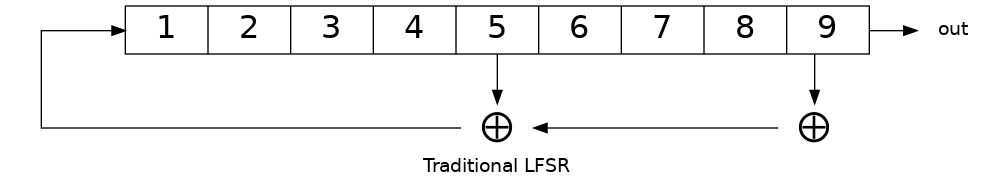
\includegraphics[width=0.7\linewidth]{img/m17-traditional-lfsr}
	\caption{Traditional form LFSR}
	\label{fig:m17-traditional-lfsr}
\end{figure}

However, the M17 LFSR is a slightly different. The M17 PRBS9 uses the generated bit as the output bit rather than the high-bit before the shift.

\begin{figure}[H]
	\centering
	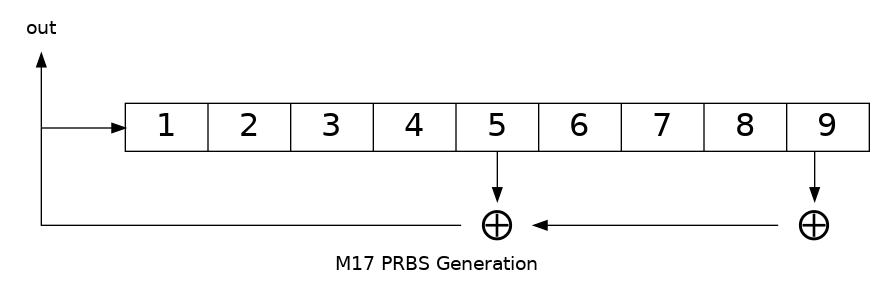
\includegraphics[width=0.7\linewidth]{img/m17-prbs9}
	\caption{M17 LFSR}
	\label{fig:m17-prbs9}
\end{figure}

This will result in the same sequence, just shifted by nine bits.

${M17\_PRBS}_{n} = {PRBS9}_{n + 8}$

The reason for this is that it allows for easier synchronization. This is equivalent to a multiplicative scrambler (a self-synchronizing scrambler) fed with a stream of 0s.

\begin{figure}[H]
	\centering
	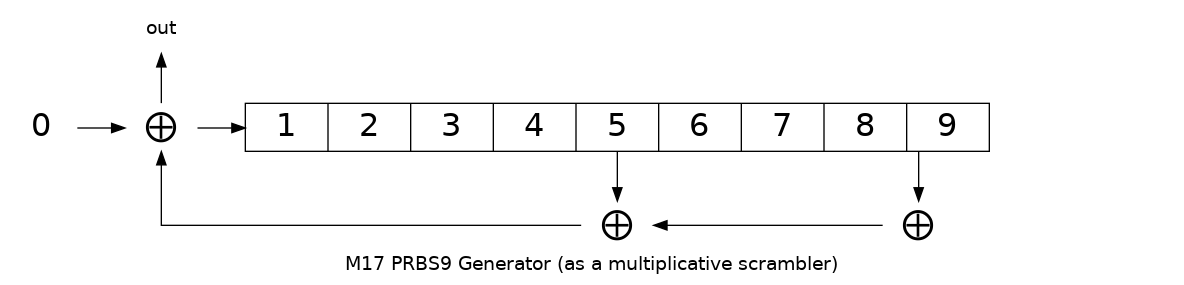
\includegraphics[width=0.7\linewidth]{img/m17-equivalent-scrambler}
	\caption{M17 PRBS9 Generator}
	\label{fig:m17-equivalent-scrambler}
\end{figure}

\begin{lstlisting}[language=C]
	class PRBS9 {
		static constexpr uint16_t MASK = 0x1FF;
		static constexpr uint8_t TAP_1 = 8;       // Bit 9
		static constexpr uint8_t TAP_2 = 4;       // Bit 5
		
		uint16_t state = 1;
		
		public:
		bool generate()
		{
			bool result = ((state >> TAP_1) ^ (state >> TAP_2)) & 1;
			state = ((state << 1) | result) & MASK;
			return result;
		}
		...
	};
\end{lstlisting}

The PRBS9 SHOULD be initialized with a state of 1.

\section{PRBS Receiver}

The receiver detects the frame is a BERT Frame based on the Sync Burst received. If the PRBS9 generator is reset at this point, the sender and receiver should be synchronized at the start. This, however, is not common nor is it required. PRBS generators can be self-synchronizing.

\subsection{Synchronization}

The receiver will synchronize the PRBS by first XORing the received bit with the LFSR taps. If the result of the XOR is a 1, it is an error (the expected feedback bit and the input do not match) and the sync count is reset. The received bit is then also shifted into the LFSR state register. Once a sequence of eighteen (18) consecutive good bits are recovered (twice the length of the LFSR), the stream is considered synchronized.

\begin{figure}[H]
	\centering
	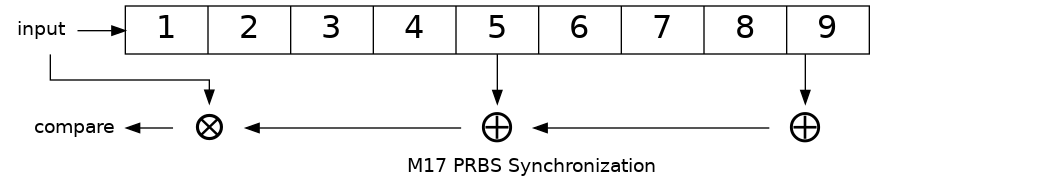
\includegraphics[width=0.7\linewidth]{img/m17-prbs9-sync}
	\caption{M17 PRBS9 Synchronization}
	\label{fig:m17-prbs9-sync}
\end{figure}

During synchronization, bits received and bit errors are not counted
towards the overall bit error rate.

\begin{lstlisting}[language=C]
	class PRBS9 {
		...
		static constexpr uint8_t LOCK_COUNT = 18;   // 18 consecutive good bits.
		...
		// PRBS Synchronizer. Returns 0 if the bit matches the PRBS, otherwise 1.
		// When synchronizing the LFSR used in the PRBS, a single bad input bit
		// will result in 3 error bits being emitted, one for each tap in the LFSR.
		bool synchronize(bool bit)
		{
			bool result = (bit ^ (state >> TAP_1) ^ (state >> TAP_2)) & 1;
			state = ((state << 1) | bit) & MASK;
			if (result) {
				sync_count = 0; // error
			} else {
				if (++sync_count == LOCK_COUNT) {
					synced = true;
					...
				}
			}
			return result;
		}
		...
	};
\end{lstlisting}

\subsection{Counting Bit Errors}

After synchronization, BERT mode switches to error-counting mode, where the received bits are compared to a free-running PRBS9 generator. Each bit that does not match the output of the free-running LFSR is counted as a bit error.

\begin{figure}[H]
	\centering
	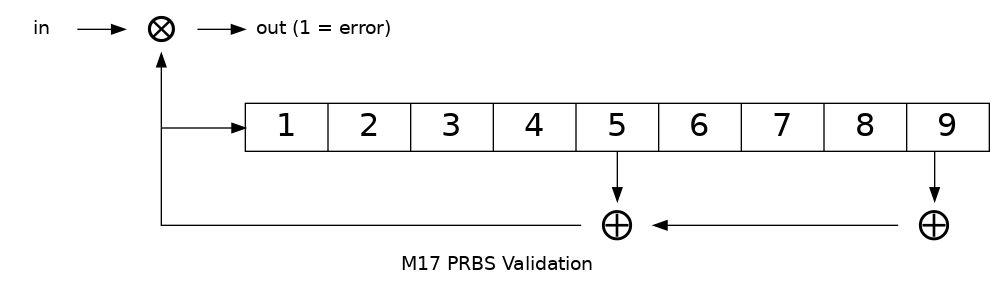
\includegraphics[width=0.7\linewidth]{img/m17-prbs9-validation}
	\caption{M17 PRBS9 Validation}
	\label{fig:m17-prbs9-validation}
\end{figure}

\begin{lstlisting}[language=C]
	class PRBS9 {
		...
		// PRBS validator.  Returns 0 if the bit matches the PRBS, otherwise 1.
		// The results are only valid when sync() returns true;
		bool validate(bool bit)
		{
			bool result;
			if (!synced) {
				result = synchronize(bit);
			} else {
				// PRBS is now free-running.
				result = bit ^ generate();
				count_errors(result);
			}
			return result;
		}
		...
	};
\end{lstlisting}

\subsection{Resynchronization}

The receiver must keep track of the number of bit errors over a period of 128 bits. If more than 18 bit errors occur, the synchronization process starts anew. This is necessary in the case of missed frames or other serious synchronization issues.

Bits received and errors which occur during resynchronization are not counted towards the bit error rate.

\section{References}

\begin{itemize}
	\item
	\href{http://www.itu.int/rec/T-REC-O.150-199210-S}{ITU O.150 : Digital 	test patterns for performance measurements on digital transmission 	equipment}
	\item
	\href{http://www.pldworld.com/_hdl/5/-thorsten-gaertner.de/vhdl/PRBS.pdf}{PRBS
	(according ITU-T O.150) and Bit-Sequence Tester : VHDL-Modules}
\end{itemize}

\chapter{KISS Protocol}

The purpose of this appendix is to document conventions for adapting KISS TNCs to M17 packet and streaming modes. M17 is a more complex protocol, both at the baseband level and at the data link layer than is typical for HDLC-based protocols commonly used on KISS TNCs. However, it is well suited for modern packet data links, and can even be used to stream digital audio between a host and a radio.

This appendix assumes the reader is familiar with the streaming and packet modes defined in the M17 spec, and with KISS TNCs and the KISS protocol.

In all cases, the TNC expects to get the data payload to be sent and is responsible for frame construction, FEC encoding, puncturing, interleaving and decorrelation. It is also responsible for baseband modulation.

For streaming modes, all voice encoding (Codec2) is done on the host and not on the TNC. The host is also responsible for constructing the LICH.

\section{Glossary}

\subsection{TNC}

Terminal node controller -- a baseband network interface device to allow host computers to send data over a radio network, similar to a modem. It connects a computer to a radio and handles the baseband portion of the physical layer and the data link layer of network protocol stack.

\subsection{KISS}

Short for ``Keep it simple, stupid''. A simplified TNC protocol designed to move everything except for the physical layer and the data link layer out of the TNC. Early TNCs could include everything up through the application layer of the OSI network model.

\subsection{SLIP}

\href{https://en.wikipedia.org/wiki/Serial_Line_Internet_Protocol}{Serial Line Internet Protocol} -- the base protocol used by the KISS protocol, extended by adding a single \textbf{type indicator} byte at the start of a frame.

\subsection{type indicator}

A one byte code at the beginning of a KISS frame which indicates the TNC \textbf{port} and KISS \textbf{command}. 

\subsection{port}

A logical port on a TNC. This allowed a single TNC to connect to multiple radios. Its specific use is loosely defined in the KISS spec. The high nibble of the KISS \textbf{type indicator}. Port 0xF is reserved.

\subsection{command}

A KISS command. This tells the TNC or host how to interpret the KISS frame contents. The low nibble of the KISS \textbf{type indicator}. Command 0xF is reserved.

\subsection{CSMA}

\href{https://en.wikipedia.org/wiki/Carrier-sense_multiple_access}{Carrier-sense multiple access} -- a protocol used by network devices to minimize collisions on a shared communications channel.

\subsection{HDLC}

\href{https://en.wikipedia.org/wiki/High-Level_Data_Link_Control}{High-Level Data Link Control} -- a data link layer framing protocol used in many AX.25 packet radio networks. Many existing protocol documents, including KISS, reference HDLC because of its ubiquity when the protocols were invented. However, HDLC is not a requirement for higher level protocols like KISS which are agnostic to the framing used at the data link layer.

\subsection{EOS}

End of stream -- an indicator bit in the frame number field of a stream data frame.

\subsection{LICH}

Link information channel -- a secondary data channel in the stream data frame containing supplemental information, including a copy of the link setup frame.

\section{M17 Protocols}

This specification defines KISS TNC modes for M17 packet and streaming modes, allowing the KISS protocol to be used to send and receive M17 packet and voice data. Both are bidirectional. There are two packet modes defined. This is done to provide complete access to the M17 protocol while maintaining the greatest degree of backwards compatibility with existing packet applications.

These protocols map to specific KISS port. The host tells the TNC what type of data to transmit based on the port used in host to TNC transfers. And the TNC tells the host what data it has received by the port set on TNC to host transfers.

This document outlines first the two packet protocols, followed by the streaming protocol.

\section{KISS Basics}

\subsection{TX Delay}

If a \textbf{KISS TX} delay $T_d$ greater than 0 is specified, the transmitter is keyed for $T_d \times 10ms$ with only a DC signal present.

The $T_d$ value should be adjusted to the minimum required by the
transmitter in order to transmit the full preamble reliably.

Only a single 40ms preamble frame is ever sent.

\begin{quote}
	NOTE A TX delay may be necessary because many radios require some 	time between when PTT is engaged and the transmitter can begin 	transmitting a modulated signal.
\end{quote}

\section{Packet Protocols}

In order to provide backward compatibility with the widest range of existing ham radio software, and to make use of features in the the M17 protocol itself, we will define two distinct packet interfaces BASIC and FULL.

The KISS protocol allows us to target specific modems using the port identifier in the control byte.

We first define basic packet mode as this is initially likely to be the most commonly used mode over KISS.

\subsection{M17 Basic Packet Mode}

Basic packet mode uses only the standard KISS protocol on TNC port 0. This is the default port for all TNCs. Packets are sent using command 0. Again, this is normal behavior for KISS client applications.

\paragraph{Sending Data}

In basic mode, the TNC only expects to receive packets from the host, as it would for any other mode supported AFSK, G3RUH, etc.

If the TNC is configured for half-duplex, the TNC will do P-persistence CSMA using a 40ms slot time and obey the P value set via the KISS interface. CSMA is disabled in full-duplex mode.

The \textbf{TX Tail} value is deprecated and is ignored.

The TNC sends the preamble burst.

The TNC is responsible for constructing the link setup frame, identifying the content as a raw mode packet. The source field is an encoded TNC identifier, similar to the APRS TOCALL, but it can be an arbitrary text string up to 9 characters in length. The destination is set to the broadcast address.

In basic packet mode, it is expected that the sender callsign is embedded within the packet payload.

The TNC sends the link setup frame.

The TNC then computes the CRC for the full packet, splits the packet into data frames encode and modulate each frame back-to-back until the packet is completely transmitted.

If there is another packet to be sent, the preamble can be skipped and the TNC will construct the next link setup frame (it can re-use the same link setup frame as it does not change) and send the next set of packet frames.

\paragraph{Limitations}

The KISS specification defines no limitation to the packet size allowed. Nor does it specify any means of returning error conditions back to the host. M17 packet protocol limits the raw packet payload size to 798 bytes. The TNC must drop any packets larger than this.

\paragraph{Receiving Data}

When receiving M17 data, the TNC must receive and parse the link setup frame and verify that the following frames contain raw packet data.

The TNC is responsible for decoding each packet, assembling the packet from the sequence of frames received, and verifying the packet checksum. If the checksum is valid, the TNC transfers the packet, excluding the CRC to the host using \textbf{KISS port} 0.

\subsection{M17 Full Packet Mode}

The purpose of full packet mode is to provide access to the entire M17 packet protocol to the host. This allows the host to set the source and destination fields, filter received packets based on the content these fields, enable encryption, and send and receive type-coded frames.

Use M17 full packet mode by sending to \textbf{KISS port} 1. In this mode the host is responsible for sending both the link setup frame and the packet data. It does this by prepending the 30-byte link setup frame to the packet data, sending this to the TNC in a single KISS frame. The TNC uses the first 30 bytes as the link setup frame verbatim, then splits the remaining data into M17 packet frames.

As with basic mode, the TNC uses the \textbf{Duplex} setting to enable/disable CSMA, and uses the \textbf{P value} for CSMA, with a fixed slot time of ``4'' (40 ms).

\paragraph{Receiving Data}

For TNC to host transfers, the same occurs. The TNC combines the link setup frame with the packet frame and sends both in one KISS frame to the host using \textbf{KISS port} 1.

\section{Stream Protocol}

The streaming protocol is fairly trivial to describe. It is used by sending first a link setup frame followed by a stream of 26-byte data frames to KISS port 2.

\subsection{Stream Format}

\paragraph{M17 KISS Stream Protocol}

\begin{table}[H]
	\centering
	\begin{tblr}{
		colspec={lX},
		}
		\hline
		Frame Size & Contents \\
		\hline
		30 & Link Setup Frame \\
		26 & LICH + Payload \\
		26 & LICH + Payload \\
		\ldots{} & \ldots{} \\
		26 & LICH + Payload with EOS bit set \\
		\hline[2px]
	\end{tblr}
	\caption{KISS Stream}
\end{table}

The host must not send any frame to any other KISS port while a stream is active (a frame with the EOS bit has not been sent).

It is a protocol violation to send anything other than a link setup frame with the stream mode bit set in the first field as the first frame in a stream transfer to KISS port 2. Any such frame is ignored.

It is a protocol violation to send anything to any other KISS port while a stream is active. If that happens the stream is terminated and the packet that caused the protocol violation is dropped.

\subsection{Data Frames}

The data frames contain a 6-byte (48-bit) LICH segment followed by a 20 byte payload segment consisting of frame number, 16-byte data payload and CRC. The TNC is responsible for parsing the frame number and detecting the end-of- stream bit to stop transmitting.

\paragraph{KISS Stream Data Frame}

\begin{table}[H]
	\centering
	\begin{tblr}{
		colspec={lX},
		}
		\hline
		Frame Size & Contents \\
		\hline
		6 & LICH (48 bits) \\
		2 & Frame Number and EOS Flag \\
		16 & Payload \\
		2 & M17 CRC of frame number and payload \\
		\hline[2px]
	\end{tblr}
	\caption{KISS Stream Data}
\end{table}

The TNC is responsible for FEC-encoding both the LICH the payload, as well as interleaving, decorrelation, and baseband modulation.

\subsection{Timing Constraints}

Streaming mode provides additional timing constraints on both host to TNC transfers and on TNC to host transfers. Payload frames must arrive every 40ms and must have a jitter below 40ms. In general, it is expected that the TNC has up to 2 frames buffered (buffering occurs while sending the preamble and link setup frames), it should be able to keep the transmit buffers filled with packet jitter of 40ms.

The TNC must stop transmitting if the transmit buffers are empty. The TNC communicates that it has stopped transmitting early (before seeing a frame with the end of stream indicator set) by sending an empty data frame to the host.

\section{TNC to Host Transfers}

TNC to host transfers are similar in that the TNC first sends the 30-byte link setup frame received to the host, followed by a stream of 26-byte data frames as described above. These are sent using \textbf{KISS port} 2.

The TNC must send the link setup frame first. This means that the TNC must be able to decode LICH segments and assemble a valid link setup frame before it sends the first data frame. The TNC will only send a link setup frame with a valid CRC to the host. After the link setup frame is sent, the TNC ignores the CRC and sends all valid frames (those received after a valid sync word) to the host. If the stream is lost before seeing an end-of-stream flag, the TNC sends a 0-byte data frame to indicate loss of signal.

The TNC must then re-acquire the signal by decoding a valid link setup frame from the LICH in order to resume sending to the host.

\section{Busy Channel Lockout}

The TNC implements \textbf{busy channel lockout} by enabling half-duplex mode on the TNC, and disables \textbf{busy channel lockout} by enabling full-duplex mode. When busy channel lockout occurs, the TNC keeps the link setup frame and discards all data frames until the channel is available. It then sends the preamble, link setup frame, and starts sending the data frames as they are received.

\begin{quote}
	NOTE BCL will be apparent to a receiver as the first frame received after the link setup frame will not start with frame number 0.
\end{quote}

\subsection{Limitations}

Information is lost by having the TNC decode the LICH. It is not possible to communicate to the host that the LICH bytes are known to be invalid.

Should we have the TNC signal the host by dropping known invalid LICH segments? The host can tell that the LICH is missing by looking at the frame size.

\section{Mixing Modes}

An M17 KISS TNC need not keep track of state across distinct TNC ports. Packet transfers are sent one packet at a time. It is OK to send to port 0 and port 1 in subsequent transfers. It is also OK to send a packet followed immediately by a voice streams. As mentioned earlier, it is a protocol violation to sent a KISS frame to any other port while a stream is active. However, a packet can be sent immediately following a voice stream (after EOS is sent).

\subsection{Back-to-back Transfers}

The TNC is expected to detect back-to-back transfers from the host, even across different KISS ports, and suppress the generation of the preamble.

For example, a packet containing APRS data sent immediately on PTT key-up should be sent immediately after the EOS frame.

Back-to-back transfers are common for packet communication where the window size determines the number of unacknowledged frames which may be outstanding (unacknowledged). Packet applications will frequently send back-to-back packets (up to window size packets) before waiting for the remote end to send ACKs for each of the packets.

\section{Implementation Details}

\subsection{Polarity}

One of the issues that must be addressed by the TNC designer, and one which the KISS protocol offers no ready solution for, is the issue of polarity.

A TNC must interface with a RF transceiver for a complete M17 physical layer implementation. RF transceivers may have different polarity for their TX and RX paths.

M17 defines that the +3 symbol is transmitted with a +2.4 kHz deviation (2.4 kHz above the carrier). \textbf{Normal polarity} in a transceiver results in a positive voltage driving the frequency higher and a lower voltage driving the frequency lower. \textbf{Reverse polarity} is the opposite. A higher voltage drives the frequency lower.

On the receive side the same issue exists. \textbf{Normal polarity} results in a positive voltage output when the received signal is above the carrier frequency. \textbf{Reverse polarity} results in a positive voltage when the frequency is below the carrier.

Just as with transmitter deviation levels and received signal levels, the polarity of the transmit and receive path must be adjustable on a 4-FSK modem. The way these adjustments are made to the TNC are not addressed by the KISS specification.

\chapter{File Formats}

This appendix documents the file formats used for testing various M17
layers.

\section{Glossary}

\subsection{Bit numbering, Bit order, Most significant bit (MSB), Least significant bit (LSB)}

\href{https://en.wikipedia.org/wiki/Bit_numbering}{Bit numbering} is how bit positions are identified in a binary number. The least significant bit (LSB) is the bit position representing a value of 1. The most significant bit (MSB) is the bit position representing the highest value position. Bit order refers to the order in which bits are extracted from a binary number. This is important especially when sending binary values one bit at a time, or when constructing multiple-bit symbols. LSB first means the extraction happens from the least significant position first. MSB first means extraction happens from the most significant position first.

\subsection{Deviation, Frequency Deviation}

In this context, deviation how far from the center frequency a carrier is shifted. This can be positive or negative. For M17, the frequency deviation of the four symbols are shown in Physical Layer Table 1.

\subsection{Deviation Function (Transmit)}

A function used to convert symbol values to frequency deviation in RF hardware. This can be used to set hardware registers, create voltages, etc. depending on the hardware used.

\subsection{Deviation Function (Receive)}

A function used to convert frequency deviation in RF hardware to symbol values. This can be used when reading hardware registers, sampling voltages, etc. depending on the hardware used.

\subsection{Dibit}

Two bits used to represent a symbol, as shown in Physical Layer Table 1.

\subsection{Endianness, Byte order, Big-endian (BE), Little-endian (LE)}

\href{https://en.wikipedia.org/wiki/Endianness}{Endianness} is the order of the bytes in a word of digital data. In this document, we will refer to big-endian (BE) and little-endian (LE). BE means that the most significant byte of a word is at the lowest memory location, while LE means that the least significant byte is at the lowest memory location.

\subsection{RF Sample Rate}

The rate at which deviation values are updated. This will vary depending on the hardware. M17 test software commonly uses 48000 samples per second.

\subsection{Root-raised-cosine (RRC) Filter}

A filter used to in digital communications to help reduce intersymbol interference. The M17 Physical Layer specifies a root-raised-cosine (RRC) filter with alpha = 0.5 \href{https://en.wikipedia.org/wiki/Root-raised-cosine_filter}{Root
Raised Cosine}

\subsection{Symbol}

An M17 Physical Layer symbol of +3, +1, -1, and -3.

\subsection{Symbol Rate}

The rate at which new symbols are generated. For M17, this is 4800 symbols per second.

\section{File Extensions}

Multiple files are used when testing the different elements of the M17 protocol. File extensions (the three characters after a period in a complete file name) are defined to standardize formats and usage.

\begin{table}[H]
	\begin{tblr}{
		colspec={lXlX},
		}
		\hline
		Extension & Description & Data Format &	Data Rate \\
		\hline
		aud & Mono audio & Signed 16-bit LE & 8000 samples per second \\
		sym & M17 symbols & Signed 8-bit & 4800 symbols per second \\
		bin & Packed M17 Dibits & MSB first, Unsigned 8-bit & 4800 symbols per
		second (1200 bytes per second) \\
		rrc & RRC filtered and Scaled M17 symbols & Signed 16-bit LE & 48000
		samples per second \\
		dev & Deviation values & Varies & Varies \\
		\hline[2px]
	\end{tblr}
	\caption{File extensions}
\end{table}

\subsection{aud}

Mono audio of signed 16-bit LE at a rate of 8000 samples per second. This is often referred to as a ``raw'' audio file and contains no embedded header information.

\subsection{sym}

M17 symbols (+3, +1, -1, -3) encoded as signed 8-bit values at rate of 4800 symbols per second.

\subsection{bin}

M17 symbols packed 2 bits per symbol (dibits), 4 symbols per byte (+3 = 01, +1 = 00, -1 = 10, -3 = 11) with the MSB first. These are unsigned 8-bit values at 4800 symbols per second, which is 4 symbols per byte at 1200 bytes per second.

\subsection{rrc}

RRC filtered and scaled M17 symbols. In order to generate a reasonable RRC waveform, the symbol rate (4800 symbols per second) is upsampled by a factor of 10 to an RRC sample rate of 48000 samples per second. Then the upsampled symbols are passed through the RRC filter. The output samples of the RRC filter are multiplied by 7168 to fit within a signed 16-bit LE representation (e.g.~a +3 value would be +21504).

\subsection{dev}

Hardware specific deviation values. These would be obtained by passing RRC filtered values through a deviation function. Since these are device specific, it is recommended to use an underscore plus device type as part of the filename. For example, the Semtech SX1276 uses a deviation step size of 61 Hz per bit. An M17 1600 Hz frequency step is equivalent to an SX1276 deviation value change of 26. Since the SX1276 only accepts positive deviation steps, the deviation function for the SX1276 would be (rrc value + 3.0) x 13. The .dev file specific for the SX1276 would contain those values, and could have a name such as m17test\_sx1276.dev

\section{Example file flows}

These show the file types in order of processing for transmit and receive flows. Each ``-\textgreater{}'' symbolizes processing required to move from one file type to the next.

\subsection{Transmit}

aud -\textgreater{} sym -\textgreater{} rrc -\textgreater{} dev

aud -\textgreater{} bin -\textgreater{} rrc -\textgreater{} dev

\subsection{Receive}

dev -\textgreater{} rrc -\textgreater{} sym -\textgreater{} aud

dev -\textgreater{} rrc -\textgreater{} bin -\textgreater{} aud

\section{To-Do}

File formats for packet and voice + data streams. 


\section{References}

\href{https://en.wikipedia.org/wiki/Bit_numbering}{Bit numbering}

\href{https://en.wikipedia.org/wiki/Endianness}{Endianness}

\href{https://en.wikipedia.org/wiki/Root-raised-cosine_filter}{Root
Raised Cosine}

\chapter{GNU Free Documentation License}
\phantomsection  % so hyperref creates bookmarks
%\addcontentsline{toc}{chapter}{GNU Free Documentation License}
%\label{label_fdl}

\begin{center}
	
	Version 1.3, 3 November 2008
	
	
	Copyright \copyright{} 2000, 2001, 2002, 2007, 2008  Free Software Foundation, Inc.
	
	\bigskip
	
	\texttt{<https://fsf.org/>}
	
	\bigskip
	
	Everyone is permitted to copy and distribute verbatim copies
	of this license document, but changing it is not allowed.
\end{center}


\begin{center}
	{\bf\large Preamble}
\end{center}

The purpose of this License is to make a manual, textbook, or other
functional and useful document ``free'' in the sense of freedom: to
assure everyone the effective freedom to copy and redistribute it,
with or without modifying it, either commercially or noncommercially.
Secondarily, this License preserves for the author and publisher a way
to get credit for their work, while not being considered responsible
for modifications made by others.

This License is a kind of ``copyleft'', which means that derivative
works of the document must themselves be free in the same sense.  It
complements the GNU General Public License, which is a copyleft
license designed for free software.

We have designed this License in order to use it for manuals for free
software, because free software needs free documentation: a free
program should come with manuals providing the same freedoms that the
software does.  But this License is not limited to software manuals;
it can be used for any textual work, regardless of subject matter or
whether it is published as a printed book.  We recommend this License
principally for works whose purpose is instruction or reference.


\begin{center}
	{\Large\bf 1. APPLICABILITY AND DEFINITIONS\par}
	\phantomsection
	\addcontentsline{toc}{section}{1. APPLICABILITY AND DEFINITIONS}
\end{center}

This License applies to any manual or other work, in any medium, that
contains a notice placed by the copyright holder saying it can be
distributed under the terms of this License.  Such a notice grants a
world-wide, royalty-free license, unlimited in duration, to use that
work under the conditions stated herein.  The ``\textbf{Document}'', below,
refers to any such manual or work.  Any member of the public is a
licensee, and is addressed as ``\textbf{you}''.  You accept the license if you
copy, modify or distribute the work in a way requiring permission
under copyright law.

A ``\textbf{Modified Version}'' of the Document means any work containing the
Document or a portion of it, either copied verbatim, or with
modifications and/or translated into another language.

A ``\textbf{Secondary Section}'' is a named appendix or a front-matter section of
the Document that deals exclusively with the relationship of the
publishers or authors of the Document to the Document's overall subject
(or to related matters) and contains nothing that could fall directly
within that overall subject.  (Thus, if the Document is in part a
textbook of mathematics, a Secondary Section may not explain any
mathematics.)  The relationship could be a matter of historical
connection with the subject or with related matters, or of legal,
commercial, philosophical, ethical or political position regarding
them.

The ``\textbf{Invariant Sections}'' are certain Secondary Sections whose titles
are designated, as being those of Invariant Sections, in the notice
that says that the Document is released under this License.  If a
section does not fit the above definition of Secondary then it is not
allowed to be designated as Invariant.  The Document may contain zero
Invariant Sections.  If the Document does not identify any Invariant
Sections then there are none.

The ``\textbf{Cover Texts}'' are certain short passages of text that are listed,
as Front-Cover Texts or Back-Cover Texts, in the notice that says that
the Document is released under this License.  A Front-Cover Text may
be at most 5 words, and a Back-Cover Text may be at most 25 words.

A ``\textbf{Transparent}'' copy of the Document means a machine-readable copy,
represented in a format whose specification is available to the
general public, that is suitable for revising the document
straightforwardly with generic text editors or (for images composed of
pixels) generic paint programs or (for drawings) some widely available
drawing editor, and that is suitable for input to text formatters or
for automatic translation to a variety of formats suitable for input
to text formatters.  A copy made in an otherwise Transparent file
format whose markup, or absence of markup, has been arranged to thwart
or discourage subsequent modification by readers is not Transparent.
An image format is not Transparent if used for any substantial amount
of text.  A copy that is not ``Transparent'' is called ``\textbf{Opaque}''.

Examples of suitable formats for Transparent copies include plain
ASCII without markup, Texinfo input format, LaTeX input format, SGML
or XML using a publicly available DTD, and standard-conforming simple
HTML, PostScript or PDF designed for human modification.  Examples of
transparent image formats include PNG, XCF and JPG.  Opaque formats
include proprietary formats that can be read and edited only by
proprietary word processors, SGML or XML for which the DTD and/or
processing tools are not generally available, and the
machine-generated HTML, PostScript or PDF produced by some word
processors for output purposes only.

The ``\textbf{Title Page}'' means, for a printed book, the title page itself,
plus such following pages as are needed to hold, legibly, the material
this License requires to appear in the title page.  For works in
formats which do not have any title page as such, ``Title Page'' means
the text near the most prominent appearance of the work's title,
preceding the beginning of the body of the text.

The ``\textbf{publisher}'' means any person or entity that distributes
copies of the Document to the public.

A section ``\textbf{Entitled XYZ}'' means a named subunit of the Document whose
title either is precisely XYZ or contains XYZ in parentheses following
text that translates XYZ in another language.  (Here XYZ stands for a
specific section name mentioned below, such as ``\textbf{Acknowledgements}'',
``\textbf{Dedications}'', ``\textbf{Endorsements}'', or ``\textbf{History}''.)  
To ``\textbf{Preserve the Title}''
of such a section when you modify the Document means that it remains a
section ``Entitled XYZ'' according to this definition.

The Document may include Warranty Disclaimers next to the notice which
states that this License applies to the Document.  These Warranty
Disclaimers are considered to be included by reference in this
License, but only as regards disclaiming warranties: any other
implication that these Warranty Disclaimers may have is void and has
no effect on the meaning of this License.


\begin{center}
	{\Large\bf 2. VERBATIM COPYING\par}
	\phantomsection
	\addcontentsline{toc}{section}{2. VERBATIM COPYING}
\end{center}

You may copy and distribute the Document in any medium, either
commercially or noncommercially, provided that this License, the
copyright notices, and the license notice saying this License applies
to the Document are reproduced in all copies, and that you add no other
conditions whatsoever to those of this License.  You may not use
technical measures to obstruct or control the reading or further
copying of the copies you make or distribute.  However, you may accept
compensation in exchange for copies.  If you distribute a large enough
number of copies you must also follow the conditions in section~3.

You may also lend copies, under the same conditions stated above, and
you may publicly display copies.


\begin{center}
	{\Large\bf 3. COPYING IN QUANTITY\par}
	\phantomsection
	\addcontentsline{toc}{section}{3. COPYING IN QUANTITY}
\end{center}


If you publish printed copies (or copies in media that commonly have
printed covers) of the Document, numbering more than 100, and the
Document's license notice requires Cover Texts, you must enclose the
copies in covers that carry, clearly and legibly, all these Cover
Texts: Front-Cover Texts on the front cover, and Back-Cover Texts on
the back cover.  Both covers must also clearly and legibly identify
you as the publisher of these copies.  The front cover must present
the full title with all words of the title equally prominent and
visible.  You may add other material on the covers in addition.
Copying with changes limited to the covers, as long as they preserve
the title of the Document and satisfy these conditions, can be treated
as verbatim copying in other respects.

If the required texts for either cover are too voluminous to fit
legibly, you should put the first ones listed (as many as fit
reasonably) on the actual cover, and continue the rest onto adjacent
pages.

If you publish or distribute Opaque copies of the Document numbering
more than 100, you must either include a machine-readable Transparent
copy along with each Opaque copy, or state in or with each Opaque copy
a computer-network location from which the general network-using
public has access to download using public-standard network protocols
a complete Transparent copy of the Document, free of added material.
If you use the latter option, you must take reasonably prudent steps,
when you begin distribution of Opaque copies in quantity, to ensure
that this Transparent copy will remain thus accessible at the stated
location until at least one year after the last time you distribute an
Opaque copy (directly or through your agents or retailers) of that
edition to the public.

It is requested, but not required, that you contact the authors of the
Document well before redistributing any large number of copies, to give
them a chance to provide you with an updated version of the Document.


\begin{center}
	{\Large\bf 4. MODIFICATIONS\par}
	\phantomsection
	\addcontentsline{toc}{section}{4. MODIFICATIONS}
\end{center}

You may copy and distribute a Modified Version of the Document under
the conditions of sections 2 and 3 above, provided that you release
the Modified Version under precisely this License, with the Modified
Version filling the role of the Document, thus licensing distribution
and modification of the Modified Version to whoever possesses a copy
of it.  In addition, you must do these things in the Modified Version:

\begin{itemize}
	\item[A.] 
	Use in the Title Page (and on the covers, if any) a title distinct
	from that of the Document, and from those of previous versions
	(which should, if there were any, be listed in the History section
	of the Document).  You may use the same title as a previous version
	if the original publisher of that version gives permission.
	
	\item[B.]
	List on the Title Page, as authors, one or more persons or entities
	responsible for authorship of the modifications in the Modified
	Version, together with at least five of the principal authors of the
	Document (all of its principal authors, if it has fewer than five),
	unless they release you from this requirement.
	
	\item[C.]
	State on the Title page the name of the publisher of the
	Modified Version, as the publisher.
	
	\item[D.]
	Preserve all the copyright notices of the Document.
	
	\item[E.]
	Add an appropriate copyright notice for your modifications
	adjacent to the other copyright notices.
	
	\item[F.]
	Include, immediately after the copyright notices, a license notice
	giving the public permission to use the Modified Version under the
	terms of this License, in the form shown in the Addendum below.
	
	\item[G.]
	Preserve in that license notice the full lists of Invariant Sections
	and required Cover Texts given in the Document's license notice.
	
	\item[H.]
	Include an unaltered copy of this License.
	
	\item[I.]
	Preserve the section Entitled ``History'', Preserve its Title, and add
	to it an item stating at least the title, year, new authors, and
	publisher of the Modified Version as given on the Title Page.  If
	there is no section Entitled ``History'' in the Document, create one
	stating the title, year, authors, and publisher of the Document as
	given on its Title Page, then add an item describing the Modified
	Version as stated in the previous sentence.
	
	\item[J.]
	Preserve the network location, if any, given in the Document for
	public access to a Transparent copy of the Document, and likewise
	the network locations given in the Document for previous versions
	it was based on.  These may be placed in the ``History'' section.
	You may omit a network location for a work that was published at
	least four years before the Document itself, or if the original
	publisher of the version it refers to gives permission.
	
	\item[K.]
	For any section Entitled ``Acknowledgements'' or ``Dedications'',
	Preserve the Title of the section, and preserve in the section all
	the substance and tone of each of the contributor acknowledgements
	and/or dedications given therein.
	
	\item[L.]
	Preserve all the Invariant Sections of the Document,
	unaltered in their text and in their titles.  Section numbers
	or the equivalent are not considered part of the section titles.
	
	\item[M.]
	Delete any section Entitled ``Endorsements''.  Such a section
	may not be included in the Modified Version.
	
	\item[N.]
	Do not retitle any existing section to be Entitled ``Endorsements''
	or to conflict in title with any Invariant Section.
	
	\item[O.]
	Preserve any Warranty Disclaimers.
\end{itemize}

If the Modified Version includes new front-matter sections or
appendices that qualify as Secondary Sections and contain no material
copied from the Document, you may at your option designate some or all
of these sections as invariant.  To do this, add their titles to the
list of Invariant Sections in the Modified Version's license notice.
These titles must be distinct from any other section titles.

You may add a section Entitled ``Endorsements'', provided it contains
nothing but endorsements of your Modified Version by various
parties---for example, statements of peer review or that the text has
been approved by an organization as the authoritative definition of a
standard.

You may add a passage of up to five words as a Front-Cover Text, and a
passage of up to 25 words as a Back-Cover Text, to the end of the list
of Cover Texts in the Modified Version.  Only one passage of
Front-Cover Text and one of Back-Cover Text may be added by (or
through arrangements made by) any one entity.  If the Document already
includes a cover text for the same cover, previously added by you or
by arrangement made by the same entity you are acting on behalf of,
you may not add another; but you may replace the old one, on explicit
permission from the previous publisher that added the old one.

The author(s) and publisher(s) of the Document do not by this License
give permission to use their names for publicity for or to assert or
imply endorsement of any Modified Version.


\begin{center}
	{\Large\bf 5. COMBINING DOCUMENTS\par}
	\phantomsection
	\addcontentsline{toc}{section}{5. COMBINING DOCUMENTS}
\end{center}


You may combine the Document with other documents released under this
License, under the terms defined in section~4 above for modified
versions, provided that you include in the combination all of the
Invariant Sections of all of the original documents, unmodified, and
list them all as Invariant Sections of your combined work in its
license notice, and that you preserve all their Warranty Disclaimers.

The combined work need only contain one copy of this License, and
multiple identical Invariant Sections may be replaced with a single
copy.  If there are multiple Invariant Sections with the same name but
different contents, make the title of each such section unique by
adding at the end of it, in parentheses, the name of the original
author or publisher of that section if known, or else a unique number.
Make the same adjustment to the section titles in the list of
Invariant Sections in the license notice of the combined work.

In the combination, you must combine any sections Entitled ``History''
in the various original documents, forming one section Entitled
``History''; likewise combine any sections Entitled ``Acknowledgements'',
and any sections Entitled ``Dedications''.  You must delete all sections
Entitled ``Endorsements''.

\begin{center}
	{\Large\bf 6. COLLECTIONS OF DOCUMENTS\par}
	\phantomsection
	\addcontentsline{toc}{section}{6. COLLECTIONS OF DOCUMENTS}
\end{center}

You may make a collection consisting of the Document and other documents
released under this License, and replace the individual copies of this
License in the various documents with a single copy that is included in
the collection, provided that you follow the rules of this License for
verbatim copying of each of the documents in all other respects.

You may extract a single document from such a collection, and distribute
it individually under this License, provided you insert a copy of this
License into the extracted document, and follow this License in all
other respects regarding verbatim copying of that document.


\begin{center}
	{\Large\bf 7. AGGREGATION WITH INDEPENDENT WORKS\par}
	\phantomsection
	\addcontentsline{toc}{section}{7. AGGREGATION WITH INDEPENDENT WORKS}
\end{center}


A compilation of the Document or its derivatives with other separate
and independent documents or works, in or on a volume of a storage or
distribution medium, is called an ``aggregate'' if the copyright
resulting from the compilation is not used to limit the legal rights
of the compilation's users beyond what the individual works permit.
When the Document is included in an aggregate, this License does not
apply to the other works in the aggregate which are not themselves
derivative works of the Document.

If the Cover Text requirement of section~3 is applicable to these
copies of the Document, then if the Document is less than one half of
the entire aggregate, the Document's Cover Texts may be placed on
covers that bracket the Document within the aggregate, or the
electronic equivalent of covers if the Document is in electronic form.
Otherwise they must appear on printed covers that bracket the whole
aggregate.


\begin{center}
	{\Large\bf 8. TRANSLATION\par}
	\phantomsection
	\addcontentsline{toc}{section}{8. TRANSLATION}
\end{center}


Translation is considered a kind of modification, so you may
distribute translations of the Document under the terms of section~4.
Replacing Invariant Sections with translations requires special
permission from their copyright holders, but you may include
translations of some or all Invariant Sections in addition to the
original versions of these Invariant Sections.  You may include a
translation of this License, and all the license notices in the
Document, and any Warranty Disclaimers, provided that you also include
the original English version of this License and the original versions
of those notices and disclaimers.  In case of a disagreement between
the translation and the original version of this License or a notice
or disclaimer, the original version will prevail.

If a section in the Document is Entitled ``Acknowledgements'',
``Dedications'', or ``History'', the requirement (section~4) to Preserve
its Title (section~1) will typically require changing the actual
title.


\begin{center}
	{\Large\bf 9. TERMINATION\par}
	\phantomsection
	\addcontentsline{toc}{section}{9. TERMINATION}
\end{center}


You may not copy, modify, sublicense, or distribute the Document
except as expressly provided under this License.  Any attempt
otherwise to copy, modify, sublicense, or distribute it is void, and
will automatically terminate your rights under this License.

However, if you cease all violation of this License, then your license
from a particular copyright holder is reinstated (a) provisionally,
unless and until the copyright holder explicitly and finally
terminates your license, and (b) permanently, if the copyright holder
fails to notify you of the violation by some reasonable means prior to
60 days after the cessation.

Moreover, your license from a particular copyright holder is
reinstated permanently if the copyright holder notifies you of the
violation by some reasonable means, this is the first time you have
received notice of violation of this License (for any work) from that
copyright holder, and you cure the violation prior to 30 days after
your receipt of the notice.

Termination of your rights under this section does not terminate the
licenses of parties who have received copies or rights from you under
this License.  If your rights have been terminated and not permanently
reinstated, receipt of a copy of some or all of the same material does
not give you any rights to use it.


\begin{center}
	{\Large\bf 10. FUTURE REVISIONS OF THIS LICENSE\par}
	\phantomsection
	\addcontentsline{toc}{section}{10. FUTURE REVISIONS OF THIS LICENSE}
\end{center}


The Free Software Foundation may publish new, revised versions
of the GNU Free Documentation License from time to time.  Such new
versions will be similar in spirit to the present version, but may
differ in detail to address new problems or concerns.  See
\texttt{https://www.gnu.org/licenses/}.

Each version of the License is given a distinguishing version number.
If the Document specifies that a particular numbered version of this
License ``or any later version'' applies to it, you have the option of
following the terms and conditions either of that specified version or
of any later version that has been published (not as a draft) by the
Free Software Foundation.  If the Document does not specify a version
number of this License, you may choose any version ever published (not
as a draft) by the Free Software Foundation.  If the Document
specifies that a proxy can decide which future versions of this
License can be used, that proxy's public statement of acceptance of a
version permanently authorizes you to choose that version for the
Document.


\begin{center}
	{\Large\bf 11. RELICENSING\par}
	\phantomsection
	\addcontentsline{toc}{section}{11. RELICENSING}
\end{center}


``Massive Multiauthor Collaboration Site'' (or ``MMC Site'') means any
World Wide Web server that publishes copyrightable works and also
provides prominent facilities for anybody to edit those works.  A
public wiki that anybody can edit is an example of such a server.  A
``Massive Multiauthor Collaboration'' (or ``MMC'') contained in the
site means any set of copyrightable works thus published on the MMC
site.

``CC-BY-SA'' means the Creative Commons Attribution-Share Alike 3.0
license published by Creative Commons Corporation, a not-for-profit
corporation with a principal place of business in San Francisco,
California, as well as future copyleft versions of that license
published by that same organization.

``Incorporate'' means to publish or republish a Document, in whole or
in part, as part of another Document.

An MMC is ``eligible for relicensing'' if it is licensed under this
License, and if all works that were first published under this License
somewhere other than this MMC, and subsequently incorporated in whole
or in part into the MMC, (1) had no cover texts or invariant sections,
and (2) were thus incorporated prior to November 1, 2008.

The operator of an MMC Site may republish an MMC contained in the site
under CC-BY-SA on the same site at any time before August 1, 2009,
provided the MMC is eligible for relicensing.


\begin{center}
	{\Large\bf ADDENDUM: How to use this License for your documents\par}
	\phantomsection
	\addcontentsline{toc}{section}{ADDENDUM: How to use this License for your documents}
\end{center}

To use this License in a document you have written, include a copy of
the License in the document and put the following copyright and
license notices just after the title page:

\bigskip
\begin{quote}
	Copyright \copyright{}  YEAR  YOUR NAME.
	Permission is granted to copy, distribute and/or modify this document
	under the terms of the GNU Free Documentation License, Version 1.3
	or any later version published by the Free Software Foundation;
	with no Invariant Sections, no Front-Cover Texts, and no Back-Cover Texts.
	A copy of the license is included in the section entitled ``GNU
	Free Documentation License''.
\end{quote}
\bigskip

If you have Invariant Sections, Front-Cover Texts and Back-Cover Texts,
replace the ``with \dots\ Texts.''\ line with this:

\bigskip
\begin{quote}
	with the Invariant Sections being LIST THEIR TITLES, with the
	Front-Cover Texts being LIST, and with the Back-Cover Texts being LIST.
\end{quote}
\bigskip

If you have Invariant Sections without Cover Texts, or some other
combination of the three, merge those two alternatives to suit the
situation.

If your document contains nontrivial examples of program code, we
recommend releasing these examples in parallel under your choice of
free software license, such as the GNU General Public License,
to permit their use in free software.

\chapter{GNU General Public License, version 2}

\begin{center}
	{\parindent 0in
		
		Copyright \copyright\ 1989, 1991 Free Software Foundation, Inc.
		
		\bigskip
		
		51 Franklin Street, Fifth Floor, Boston, MA  02110-1301, USA
		
		\bigskip
		
		Everyone is permitted to copy and distribute verbatim copies
		of this license document, but changing it is not allowed.
	}
\end{center}

\begin{center}
	{\bf\large Preamble}
\end{center}


The licenses for most software are designed to take away your freedom to
share and change it.  By contrast, the GNU General Public License is
intended to guarantee your freedom to share and change free software---to
make sure the software is free for all its users.  This General Public
License applies to most of the Free Software Foundation's software and to
any other program whose authors commit to using it.  (Some other Free
Software Foundation software is covered by the GNU Library General Public
License instead.)  You can apply it to your programs, too.

When we speak of free software, we are referring to freedom, not price.
Our General Public Licenses are designed to make sure that you have the
freedom to distribute copies of free software (and charge for this service
if you wish), that you receive source code or can get it if you want it,
that you can change the software or use pieces of it in new free programs;
and that you know you can do these things.

To protect your rights, we need to make restrictions that forbid anyone to
deny you these rights or to ask you to surrender the rights.  These
restrictions translate to certain responsibilities for you if you
distribute copies of the software, or if you modify it.

For example, if you distribute copies of such a program, whether gratis or
for a fee, you must give the recipients all the rights that you have.  You
must make sure that they, too, receive or can get the source code.  And
you must show them these terms so they know their rights.

We protect your rights with two steps: (1) copyright the software, and (2)
offer you this license which gives you legal permission to copy,
distribute and/or modify the software.

Also, for each author's protection and ours, we want to make certain that
everyone understands that there is no warranty for this free software.  If
the software is modified by someone else and passed on, we want its
recipients to know that what they have is not the original, so that any
problems introduced by others will not reflect on the original authors'
reputations.

Finally, any free program is threatened constantly by software patents.
We wish to avoid the danger that redistributors of a free program will
individually obtain patent licenses, in effect making the program
proprietary.  To prevent this, we have made it clear that any patent must
be licensed for everyone's free use or not licensed at all.

The precise terms and conditions for copying, distribution and
modification follow.

\begin{center}
	{\Large \sc Terms and Conditions For Copying, Distribution and
		Modification}
\end{center}


%\renewcommand{\theenumi}{\alpha{enumi}}
\begin{enumerate}
	
	\addtocounter{enumi}{-1}
	
	\item 
	
	This License applies to any program or other work which contains a notice
	placed by the copyright holder saying it may be distributed under the
	terms of this General Public License.  The ``Program'', below, refers to
	any such program or work, and a ``work based on the Program'' means either
	the Program or any derivative work under copyright law: that is to say, a
	work containing the Program or a portion of it, either verbatim or with
	modifications and/or translated into another language.  (Hereinafter,
	translation is included without limitation in the term ``modification''.)
	Each licensee is addressed as ``you''.
	
	Activities other than copying, distribution and modification are not
	covered by this License; they are outside its scope.  The act of
	running the Program is not restricted, and the output from the Program
	is covered only if its contents constitute a work based on the
	Program (independent of having been made by running the Program).
	Whether that is true depends on what the Program does.
	
	\item You may copy and distribute verbatim copies of the Program's source
	code as you receive it, in any medium, provided that you conspicuously
	and appropriately publish on each copy an appropriate copyright notice
	and disclaimer of warranty; keep intact all the notices that refer to
	this License and to the absence of any warranty; and give any other
	recipients of the Program a copy of this License along with the Program.
	
	You may charge a fee for the physical act of transferring a copy, and you
	may at your option offer warranty protection in exchange for a fee.
	
	\item
	
	You may modify your copy or copies of the Program or any portion
	of it, thus forming a work based on the Program, and copy and
	distribute such modifications or work under the terms of Section 1
	above, provided that you also meet all of these conditions:
	
	\begin{enumerate}
		
		\item 
		
		You must cause the modified files to carry prominent notices stating that
		you changed the files and the date of any change.
		
		\item
		
		You must cause any work that you distribute or publish, that in
		whole or in part contains or is derived from the Program or any
		part thereof, to be licensed as a whole at no charge to all third
		parties under the terms of this License.
		
		\item
		If the modified program normally reads commands interactively
		when run, you must cause it, when started running for such
		interactive use in the most ordinary way, to print or display an
		announcement including an appropriate copyright notice and a
		notice that there is no warranty (or else, saying that you provide
		a warranty) and that users may redistribute the program under
		these conditions, and telling the user how to view a copy of this
		License.  (Exception: if the Program itself is interactive but
		does not normally print such an announcement, your work based on
		the Program is not required to print an announcement.)
		
	\end{enumerate}
	
	
	These requirements apply to the modified work as a whole.  If
	identifiable sections of that work are not derived from the Program,
	and can be reasonably considered independent and separate works in
	themselves, then this License, and its terms, do not apply to those
	sections when you distribute them as separate works.  But when you
	distribute the same sections as part of a whole which is a work based
	on the Program, the distribution of the whole must be on the terms of
	this License, whose permissions for other licensees extend to the
	entire whole, and thus to each and every part regardless of who wrote it.
	
	Thus, it is not the intent of this section to claim rights or contest
	your rights to work written entirely by you; rather, the intent is to
	exercise the right to control the distribution of derivative or
	collective works based on the Program.
	
	In addition, mere aggregation of another work not based on the Program
	with the Program (or with a work based on the Program) on a volume of
	a storage or distribution medium does not bring the other work under
	the scope of this License.
	
	\item
	You may copy and distribute the Program (or a work based on it,
	under Section 2) in object code or executable form under the terms of
	Sections 1 and 2 above provided that you also do one of the following:
	
	\begin{enumerate}
		
		\item
		
		Accompany it with the complete corresponding machine-readable
		source code, which must be distributed under the terms of Sections
		1 and 2 above on a medium customarily used for software interchange; or,
		
		\item
		
		Accompany it with a written offer, valid for at least three
		years, to give any third party, for a charge no more than your
		cost of physically performing source distribution, a complete
		machine-readable copy of the corresponding source code, to be
		distributed under the terms of Sections 1 and 2 above on a medium
		customarily used for software interchange; or,
		
		\item
		
		Accompany it with the information you received as to the offer
		to distribute corresponding source code.  (This alternative is
		allowed only for noncommercial distribution and only if you
		received the program in object code or executable form with such
		an offer, in accord with Subsection b above.)
		
	\end{enumerate}
	
	
	The source code for a work means the preferred form of the work for
	making modifications to it.  For an executable work, complete source
	code means all the source code for all modules it contains, plus any
	associated interface definition files, plus the scripts used to
	control compilation and installation of the executable.  However, as a
	special exception, the source code distributed need not include
	anything that is normally distributed (in either source or binary
	form) with the major components (compiler, kernel, and so on) of the
	operating system on which the executable runs, unless that component
	itself accompanies the executable.
	
	If distribution of executable or object code is made by offering
	access to copy from a designated place, then offering equivalent
	access to copy the source code from the same place counts as
	distribution of the source code, even though third parties are not
	compelled to copy the source along with the object code.
	
	\item
	You may not copy, modify, sublicense, or distribute the Program
	except as expressly provided under this License.  Any attempt
	otherwise to copy, modify, sublicense or distribute the Program is
	void, and will automatically terminate your rights under this License.
	However, parties who have received copies, or rights, from you under
	this License will not have their licenses terminated so long as such
	parties remain in full compliance.
	
	\item
	You are not required to accept this License, since you have not
	signed it.  However, nothing else grants you permission to modify or
	distribute the Program or its derivative works.  These actions are
	prohibited by law if you do not accept this License.  Therefore, by
	modifying or distributing the Program (or any work based on the
	Program), you indicate your acceptance of this License to do so, and
	all its terms and conditions for copying, distributing or modifying
	the Program or works based on it.
	
	\item
	Each time you redistribute the Program (or any work based on the
	Program), the recipient automatically receives a license from the
	original licensor to copy, distribute or modify the Program subject to
	these terms and conditions.  You may not impose any further
	restrictions on the recipients' exercise of the rights granted herein.
	You are not responsible for enforcing compliance by third parties to
	this License.
	
	\item
	If, as a consequence of a court judgment or allegation of patent
	infringement or for any other reason (not limited to patent issues),
	conditions are imposed on you (whether by court order, agreement or
	otherwise) that contradict the conditions of this License, they do not
	excuse you from the conditions of this License.  If you cannot
	distribute so as to satisfy simultaneously your obligations under this
	License and any other pertinent obligations, then as a consequence you
	may not distribute the Program at all.  For example, if a patent
	license would not permit royalty-free redistribution of the Program by
	all those who receive copies directly or indirectly through you, then
	the only way you could satisfy both it and this License would be to
	refrain entirely from distribution of the Program.
	
	If any portion of this section is held invalid or unenforceable under
	any particular circumstance, the balance of the section is intended to
	apply and the section as a whole is intended to apply in other
	circumstances.
	
	It is not the purpose of this section to induce you to infringe any
	patents or other property right claims or to contest validity of any
	such claims; this section has the sole purpose of protecting the
	integrity of the free software distribution system, which is
	implemented by public license practices.  Many people have made
	generous contributions to the wide range of software distributed
	through that system in reliance on consistent application of that
	system; it is up to the author/donor to decide if he or she is willing
	to distribute software through any other system and a licensee cannot
	impose that choice.
	
	This section is intended to make thoroughly clear what is believed to
	be a consequence of the rest of this License.
	
	\item
	If the distribution and/or use of the Program is restricted in
	certain countries either by patents or by copyrighted interfaces, the
	original copyright holder who places the Program under this License
	may add an explicit geographical distribution limitation excluding
	those countries, so that distribution is permitted only in or among
	countries not thus excluded.  In such case, this License incorporates
	the limitation as if written in the body of this License.
	
	\item
	The Free Software Foundation may publish revised and/or new versions
	of the General Public License from time to time.  Such new versions will
	be similar in spirit to the present version, but may differ in detail to
	address new problems or concerns.
	
	Each version is given a distinguishing version number.  If the Program
	specifies a version number of this License which applies to it and ``any
	later version'', you have the option of following the terms and conditions
	either of that version or of any later version published by the Free
	Software Foundation.  If the Program does not specify a version number of
	this License, you may choose any version ever published by the Free Software
	Foundation.
	
	\item
	If you wish to incorporate parts of the Program into other free
	programs whose distribution conditions are different, write to the author
	to ask for permission.  For software which is copyrighted by the Free
	Software Foundation, write to the Free Software Foundation; we sometimes
	make exceptions for this.  Our decision will be guided by the two goals
	of preserving the free status of all derivatives of our free software and
	of promoting the sharing and reuse of software generally.
	
	\begin{center}
		{\Large\sc
			No Warranty
		}
	\end{center}
	
	\item
	{\sc Because the program is licensed free of charge, there is no warranty
		for the program, to the extent permitted by applicable law.  Except when
		otherwise stated in writing the copyright holders and/or other parties
		provide the program ``as is'' without warranty of any kind, either expressed
		or implied, including, but not limited to, the implied warranties of
		merchantability and fitness for a particular purpose.  The entire risk as
		to the quality and performance of the program is with you.  Should the
		program prove defective, you assume the cost of all necessary servicing,
		repair or correction.}
	
	\item
	{\sc In no event unless required by applicable law or agreed to in writing
		will any copyright holder, or any other party who may modify and/or
		redistribute the program as permitted above, be liable to you for damages,
		including any general, special, incidental or consequential damages arising
		out of the use or inability to use the program (including but not limited
		to loss of data or data being rendered inaccurate or losses sustained by
		you or third parties or a failure of the program to operate with any other
		programs), even if such holder or other party has been advised of the
		possibility of such damages.}
	
\end{enumerate}


\begin{center}
	{\Large\sc End of Terms and Conditions}
\end{center}


\pagebreak[2]

\section*{Appendix: How to Apply These Terms to Your New Programs}

If you develop a new program, and you want it to be of the greatest
possible use to the public, the best way to achieve this is to make it
free software which everyone can redistribute and change under these
terms.

To do so, attach the following notices to the program.  It is safest to
attach them to the start of each source file to most effectively convey
the exclusion of warranty; and each file should have at least the
``copyright'' line and a pointer to where the full notice is found.

\begin{quote}
	one line to give the program's name and a brief idea of what it does. \\
	Copyright (C) yyyy  name of author \\
	
	This program is free software; you can redistribute it and/or modify
	it under the terms of the GNU General Public License as published by
	the Free Software Foundation; either version 2 of the License, or
	(at your option) any later version.
	
	This program is distributed in the hope that it will be useful,
	but WITHOUT ANY WARRANTY; without even the implied warranty of
	MERCHANTABILITY or FITNESS FOR A PARTICULAR PURPOSE.  See the
	GNU General Public License for more details.
	
	You should have received a copy of the GNU General Public License
	along with this program; if not, write to the Free Software
	Foundation, Inc., 51 Franklin Street, Fifth Floor, Boston, MA  02110-1301, USA.
\end{quote}

Also add information on how to contact you by electronic and paper mail.

If the program is interactive, make it output a short notice like this
when it starts in an interactive mode:

\begin{quote}
	Gnomovision version 69, Copyright (C) yyyy  name of author \\
	Gnomovision comes with ABSOLUTELY NO WARRANTY; for details type `show w'. \\
	This is free software, and you are welcome to redistribute it
	under certain conditions; type `show c' for details.
\end{quote}


The hypothetical commands {\tt show w} and {\tt show c} should show the
appropriate parts of the General Public License.  Of course, the commands
you use may be called something other than {\tt show w} and {\tt show c};
they could even be mouse-clicks or menu items---whatever suits your
program.

You should also get your employer (if you work as a programmer) or your
school, if any, to sign a ``copyright disclaimer'' for the program, if
necessary.  Here is a sample; alter the names:

\begin{quote}
	Yoyodyne, Inc., hereby disclaims all copyright interest in the program \\
	`Gnomovision' (which makes passes at compilers) written by James Hacker. \\
	
	signature of Ty Coon, 1 April 1989 \\
	Ty Coon, President of Vice
\end{quote}


This General Public License does not permit incorporating your program
into proprietary programs.  If your program is a subroutine library, you
may consider it more useful to permit linking proprietary applications
with the library.  If this is what you want to do, use the GNU Library
General Public License instead of this License.

\end{document}

\end{document}
